%% A simple template for a term report using the Hagenberg setup 
%% based on the standard LaTeX 'report' class

%%% Magic comments for setting the correct parameters in compatible IDEs
% !TeX encoding = utf8
% !TeX program = pdflatex 
% !TeX spellcheck = en_US
% !BIB program = biber

\RequirePackage[utf8]{inputenc} % Remove when using lualatex or xelatex!
\RequirePackage{hgbpdfa}        % Creates a PDF/A-2b compliant document

\documentclass[english,notitlepage,smartquotes]{hgbreport}
% Supported options in [..]:
%    Main language: 'german' (default), 'english'
%    Conversion to typographic quotation marks: 'smartquotes'
%    Use APA citation style: 'apa'
%    Do not create a separate title page: 'notitlepage'
%    Page layout: 'oneside' (single-sided, default), 'twoside' (double-sided)
%%%-----------------------------------------------------------------------------

\graphicspath{{images/}}  % Location of images and graphics
\bibliography{references} % Biblatex bibliography file (references.bib)
% theorems, definitions, remarks etc.
\usepackage{amsthm}

\theoremstyle{definition}
\newtheorem{definition}{Definition}

\theoremstyle{definition}
\newtheorem{problem}{Problem}

\theoremstyle{remark}
\newtheorem*{remark}{Remark}

\theoremstyle{definition}
\newtheorem{example}{Example}

\theoremstyle{plain}
\newtheorem{theorem}{Theorem}[chapter]
\newtheorem{corollary}{Corollary}[theorem]
\newtheorem{lemma}{Lemma}[chapter]
\newtheorem{mini-theorem}{Mini-theorem}
\renewcommand\qedsymbol{$\blacksquare$}
% theorems, definitions, remarks etc.
% the "reflection" box
\usepackage[framemethod=tikz]{mdframed}
\theoremstyle{definition}
\newtheorem{reflection}{Reflection}
\mdfdefinestyle{reflectionbox}{
  innertopmargin=\topskip,
  roundcorner=5pt,
  linecolor=cyan,
  backgroundcolor=cyan!20,
}
\surroundwithmdframed[style=reflectionbox]{reflection}
% the "reflection" box

% long table
\usepackage{longtable}
% long table

% for algorithm description
\usepackage{algorithm}
\usepackage{algpseudocodex}
% for algorithm description
% for images etc.
\usepackage{tikz}
\newcommand*\circled[1]{\tikz[baseline=(char.base)]{
    \node[shape=circle,draw=red,inner sep=2pt] (char) {#1};}}
\newcommand*\fillcircled[2]{\tikz[baseline=(char.base)]{
    \node[shape=circle,fill=#2,draw=red,inner sep=2pt] (char) {#1};}}
% for images etc.
% color names
\usepackage[pdftex,dvipsnames]{xcolor}
% color names
% Big starting letters
\usepackage{lettrine}
% Big starting letters
% cancel terms
\usepackage{cancel}
% cancel terms

% sidebar environment https://tex.stackexchange.com/a/735167/64425
\usepackage[most]{tcolorbox}

\newtcolorbox{sidebar}{
  breakable,
  enhanced,
  frame hidden,
  interior hidden,
  size=minimal,
  left skip=8pt,
  borderline west={1pt}{-5pt}{gray}
}
% sidebar environment https://tex.stackexchange.com/a/735167/64425

% 
\usepackage{parskip}% http://ctan.org/pkg/parskip
%
% todonotes
\usepackage{xargs}                      % Use more than one optional parameter in a new commands
\usepackage[colorinlistoftodos,prependcaption,textsize=tiny]{todonotes}
\newcommandx{\tbd}[2][1=]{\todo[linecolor=orange,backgroundcolor=orange!25,bordercolor=magenta,#1]{#2}}
\newcommandx{\doubt}[2][1=]{\todo[linecolor=red,backgroundcolor=red!25,bordercolor=black,#1]{#2}}
% todonotes
% get rid of ugly borders
\hypersetup{
    colorlinks,
    linkcolor={magenta!50!black},
    citecolor={blue!50!black},
    urlcolor={blue!80!black}
}
% get rid of ugly borders

% some commands, mainly for local use
% list of theorems
\usepackage{thmtools}
% list of theorems
% label list items
\usepackage{enumitem}
% label list items
% failed proof
\newcommand{\bogusproof}{\textcolor{red}{\Huge\bf ?}}
% failed proof
% some commands, mainly for local use
%%%-----------------------------------------------------------------------------
\begin{document}
%%%-----------------------------------------------------------------------------
\author{Kedar Mhaswade}                    % Your name
\title{Linear Algebra Problem Book:\\ % Name of the course or project
			Notes and Problem Solutions}	                 % or "Project Report"
\date{04 June 2025}

%%%-----------------------------------------------------------------------------
\maketitle
%%%-----------------------------------------------------------------------------
\begin{abstract}\noindent

\bigskip
\noindent
% Use the abstract to provide a short summary of the document's contents.
\lettrine[lines=3]{T}{his} is an objective, yet personal, narrative of the author's odyssey in the enchanted land of linear algebra. It contains his notes and solutions to problems from Professor Paul Halmos's \cite{Halmos1995} \textit{Linear Algebra Problem Book}.


I like to write. I don't have an established audience, but that does not deter me from writing. However, I have often wondered why I should carefully typeset my mathematical writing using a comprehensive system like \LaTeX. First, my mathematical writing is not `research' yet, but mainly problem-solving (which does involve at least some dogged pursuit, if not research). Second, I love writing by hand! 
\begin{figure}[!h]
\begin{center}
\caption{Handwriting is fun!}
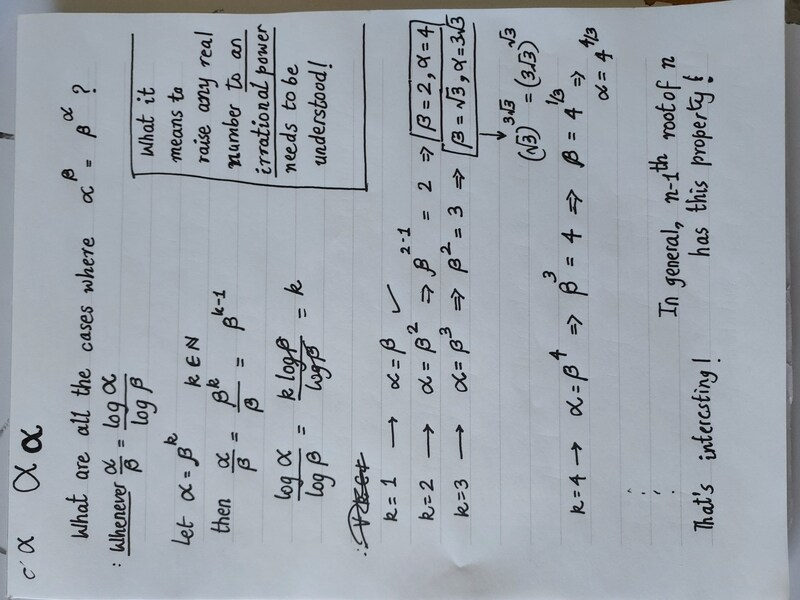
\includegraphics[width=.345\textwidth,angle=-90]{loving-to-write-by-hand-small}
\end{center}
\end{figure}

Freehand writing on a good paper with a good pen is fun. It's quick. It's rewarding.

Typesetting is, on the other hand, time-consuming and feels like \textit{Yak-shaving} \cite{Yak-shaving}. However, all good life is controlled Yak-shaving. When I typeset {\LaTeX} documents, I tend to minimize Yak-shaving and focus on having a conversation with myself. I suspect that I understand the subject matter better that way. I like the following quote in this regard:

\begin{sidebar}
I don't know what I think unless I read what I write. --Unknown
\end{sidebar}

Of course, you cannot begin solving problems on a computer. A pencil and papers are must. In this respect, typesetting is favoring form (or sophistication) over content. We strive to present beautifully what we have thought well but scribbled hastily. Fortunately, I don't mind taking the time to do that; it at least keeps me busy fine-tuning my thoughts. It sometimes even helps to find flaws.

However, the biggest advantage of typesetting my writing is keeping a record of beautifully typeset account of something, anything. If I could ever make a case to study under a stalwart like Professor Yaser Abu-Mostafa (\url{https://work.caltech.edu/}), or Professor Avrim Blum (\url{https://home.ttic.edu/~avrim/}), perhaps I can demonstrate what I have done in my scarce free time.

I have gone back and forth between handwritten pages and typeset manuscripts. However, I am resorting to typesetting for this work despite the overhead incurred. I hope I follow through. It's one thing to be motivated but another to be determined and disciplined.

Perhaps a picture (Figure [\ref{fig:mindmap}]) can explain better than words how I started reading Halmos's book. 

\begin{figure}[!h]
\begin{center}
\caption{A June 2025 Mindmap}
\label{fig:mindmap}
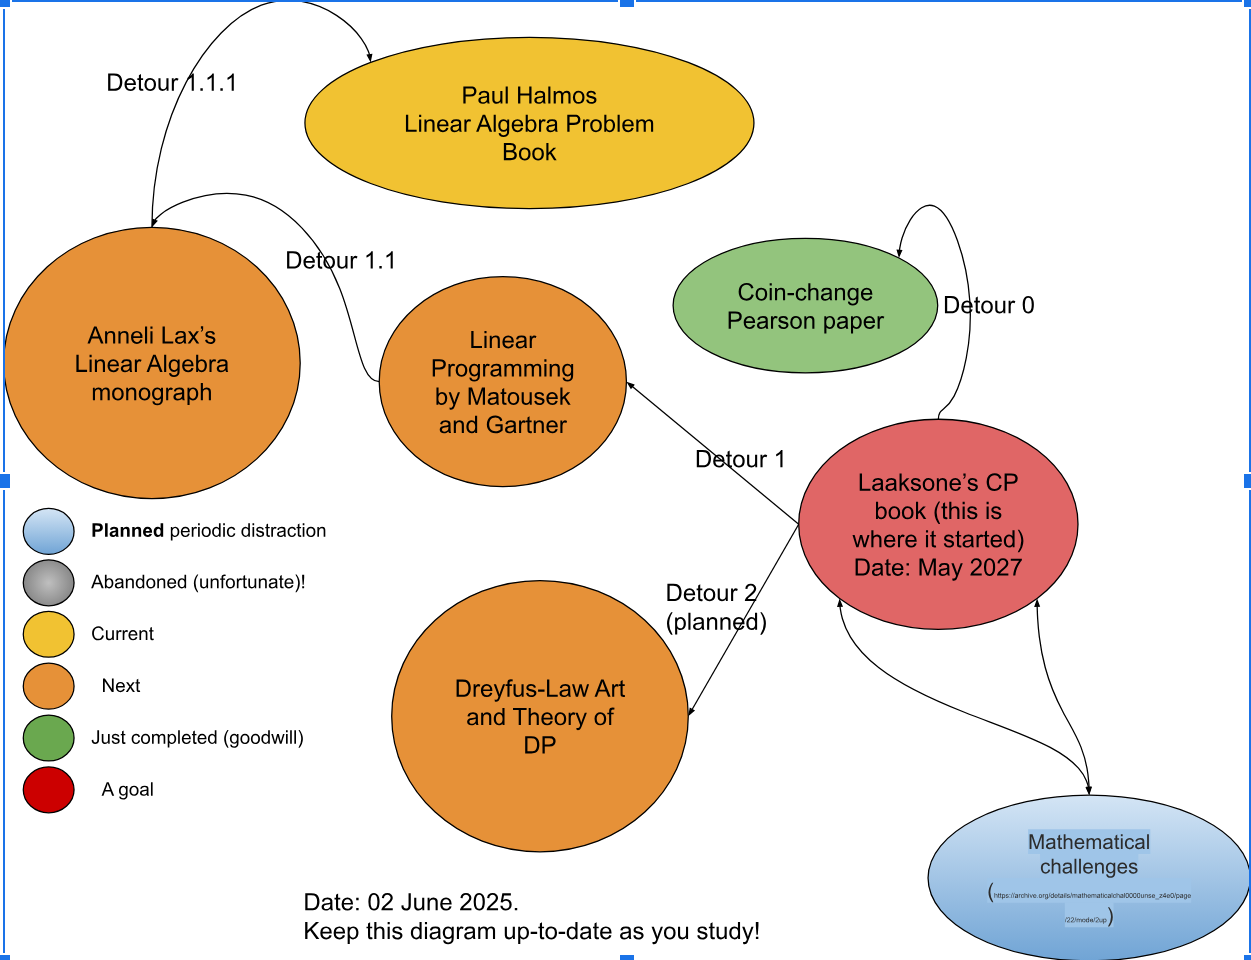
\includegraphics[width=.5\textwidth]{june-2025-mindmap}
\end{center}
\end{figure}

I will avoid answering ``Why Halmos's Linear Algebra book?''\footnote{See others' reviews of his books at \cite{ReviewsOfHalmosBooks}. All AMS reviews are by invitation only!} It suffices to say that his style resonates with me, a teaser of which can be enjoyed from what follows:

\begin{sidebar}
Is it obvious that
$$ 63+48=27+84$$?
It is a true and thoroughly uninteresting mathematical statement that can be verified in a few seconds--but is it \textit{obvious}? If calling it obvious means that the reason for its truth is clearly understood, without even a single second's verification, then most people would probably say no.

What about
$$ (27+36)+48=27+(36+84)$$
?
--is that obvious?
Yes it is, for most people; the instinctive (and correct) reaction is that the way the terms of a sum are bunched together cannot affect the answer. The approved technical term is not ``bunch together'' but ``associate''; the instinctive reaction is a readiness to accept what is called the \textbf{associative law} of addition for real numbers. (Surely every reader has noticed by now that the non-obvious statement and the obvious one are in some sense the same:

$$ 63=27+36\quad and\quad 84=36+48$$)

\textbf{Linear algebra is concerned with several different kinds of operations (such as addition) on several different kinds of objects (not necessarily real numbers)}. To prepare the ground for the study of strange operations and to keep the associative law from being unjustly dismissed as a triviality, a little effort to consider some good examples and some bad ones is worthwhile.

Some of the examples will be useful in the sequel, and some won't--some are here to show that associativity can fail, and others are here to show that even when it holds it may be far from obvious. In the world of linear algebra non-associative operations are rare, but associative operations whose good behavior is not obvious are more frequently met.

\end{sidebar}

Paul Halmos has been one of my favorite authors. His insistence on problem-solving is admirable. I hope I can painstakingly (and gleefully at the same time) solve a number of problems from this book, and understand at least some of linear algebra. The problems have been solved by Halmos himself and the answers appear at the back of this book (Thank You!), but these solutions are mine. I have also felt free to think aloud, write willfully about questions that came to my mind as I solved the stated problems. That part of writing appears like `personal reflections':
\begin{reflection}
Problems come in various levels of difficulty. And, unless you are George Dantzig (who solved an open problem written on a blackboard assuming his instructor had given a homework assignment) or the like, you have to toil through them. Some you are able to solve quickly, perhaps because you are experiencing ``flow''\footnote{A highly focused mental state, defined and popularized by the psychologist Mihaly Csikszentmihalyi, conducive to productivity}, but many are challenging and you suffer (albeit purposefully) through them. They are distinct from exercises, which are also essential for fluency and emotional well-being, but expected to be aimed at `practice' and easier to answer.
\end{reflection}
Feel free to skip them. As Halmos urges us in his preface to this book, I have read his solutions too (readily for the problems I was able to finally solve--doing so is quite important, and begrudgingly for the problems I was not able to solve in quite some time). He considers solutions an integral part of exposition. The $\blacksquare$ (QED symbol) appears after every solution. Wherever desired, I have also reinterpreted Halmos's solutions; understanding them will be certainly helpful. He has also provided hints first: Definitions, theorems, and problems, followed by hints for each problem, followed by complete solutions. There aren't very many authors who work so hard on their book!

Readable and flawless mathematical typesetting is hard. It's ironic that the epitome of exact sciences breeds a degree of inexactness in notation. Like in literature, meaning sometimes depends on context not captured in notation. And yet, an encyclopedic treatment of notation at the beginning of a work like this tends to bore readers\footnote{What disappointments them even more are typos and errors.}. Here too, a balance needs to be sought. A few conventions are therefore in order:

\begin{itemize}
\item A roman letter in italics, like, for example, $p$, generally denotes a real number, unless specified otherwise (sometimes an integer). This is different from a number theory convention. 
\item Greek letters usually denote real numbers.
\item The so-called \verb|\cdot|: $\cdot$ to denote multiplication is sometimes omitted. Thus, $ab$ is equivalent (and often even preferred and ubiquitous, thanks to Euler!) to $a\cdot b$.

\end{itemize}
\end{abstract}

%%%-----------------------------------------------------------------------------
\tableofcontents
%%%-----------------------------------------------------------------------------
% \listoftheorems % does not work TODO
\tbd{List of problems}{Fix}
%%%-----------------------------------------------------------------------------
\chapter{Scalars}
%%%-----------------------------------------------------------------------------
\begin{problem}
\label{pr:2a2b}
If a new addition for real numbers, denoted by the temporary symbol $\boxplus$, is defined by
$$
\alpha\boxplus\beta=2\alpha+2\beta
$$
, is $\boxplus$ associative?

Note: The $+$ sign on the right denotes ordinary addition.

Note: The new operation $\boxplus$ is \textit{commutative}: $\alpha\boxplus\beta=2\alpha+2\beta$ indeed equals $\beta\boxplus\alpha=2\beta+2\alpha$.
\end{problem}

\textbf{Solution}.

No. We can easily demonstrate 

$$
\alpha\boxplus(\beta\boxplus\gamma)\ne(\alpha\boxplus\beta)\boxplus\gamma
$$


\qedsymbol

\begin{problem}
\label{pr:2ab}
If a new addition for real numbers, denoted by the temporary symbol $\boxplus$, is defined by
$$
\alpha\boxplus\beta=2\alpha+\beta
$$
, is $\boxplus$ associative?
\end{problem}

\textbf{Solution}.

No. We can easily demonstrate 

$$
\alpha\boxplus(\beta\boxplus\gamma)\ne(\alpha\boxplus\beta)\boxplus\gamma
$$
\qedsymbol

\begin{problem}
\label{pr:atob}
If an operation for \emph{positive integers}, denoted by the temporary symbol $*$, is defined by
$$
\alpha*\beta=\alpha^\beta
$$
, is it commutative? Is it associative?
\end{problem}

\textbf{Solution}.

Although $\alpha^\beta=\beta^\alpha$ when $\alpha=\beta$, in general, $\alpha^{\beta}$ doesn't seem to equal $\beta^\alpha$. A simple counterexample is $\alpha=1,\beta=2$. Therefore, $*$ is not a commutative operation on two positive integers.
\qedsymbol

\begin{reflection}

I asked myself, ``For which real numbers $\alpha,\beta$ (although in Problem [\ref{pr:atob}] they are positive integers) are $\alpha^\beta$ and $\beta^\alpha$ equal?''

The following exploration amazed me.
$$
\alpha^\beta=\beta^\alpha
$$
\begin{equation}
\label{eq:takelogs}
\therefore \beta\log\alpha=\alpha\log\beta
\end{equation}

\begin{equation}
\label{eq:ablogalob}
\therefore \frac{\alpha}{\beta}=\frac{\log\alpha}{\log\beta}
\end{equation}

A general solution of equation [\ref{eq:ablogalob}] (a Diophantine equation for we seek integer solutions) is perhaps hard, but somehow I asked, ``What if $\alpha=\beta^k$ for some $k\in\mathbb N$?'' I don't know why I thought of that. Is that intuition? Maybe.

Equation [\ref{eq:ablogalob}] then gives
$$
\frac{\beta^k}{\beta}=\frac{k\cancel{\log\beta}}{\cancel{\log\beta}}
$$
which simplifies to

\begin{equation}
\label{eq:bk-1k}
\beta^{k-1}=k
\end{equation}


%\begin{table}[h!] % floats lost error!
%\centering
\begin{tabular}{|c|c|c|}
 \hline
 $k$ & What follows from $\alpha=\beta^k$ & $\alpha,\beta$ \\ \hline
 \hline
 $1$ & $\alpha=\beta$  & Any real numbers \\ \hline
 $2$ & $\beta^{2-1}=\beta=2$ & $\alpha=4,\beta=2$ \\ \hline
 $3$ & $\beta^{3-1}=\beta^2=3$ & $\alpha=3\sqrt{3},\beta=\sqrt{3}$ \\ \hline
 $4$ & $\beta^{4-1}=\beta^3=4$ & $\alpha=4\sqrt[3]{4},\beta=\sqrt[3]{4}$ \\ \hline
\end{tabular}

%\caption{When does $\alpha^\beta=\beta^\alpha$ if $\alpha=\beta^k, k\in\mathbb N$?}
%\label{tab:ab=ba}
%\end{table}

That was interesting! 

\end{reflection}

Exponentiation is associative only when $\beta\gamma=\beta^\gamma$. There are specific cases when that is true (e.g. $\beta=\gamma=2$), but it is not true in general. A simple counterexample is $\alpha=2,\beta=1,\gamma=3$.


Problem [\ref{pr:atob}] shows that ``natural'' operations can fail to be associative.

Halmos introduces complex numbers simply as a ``pair of real numbers'':$\langle\alpha,\beta\rangle\mid\alpha,\beta\in\mathbb{R}$. We can then \textit{define} operations of interest on them, and examine if they are commutative and associative.

An operation $\boxplus$ defined on complex numbers $\langle\alpha,\beta\rangle$ and $\langle\gamma,\delta\rangle$ as:

$$
\langle\alpha,\beta\rangle\boxplus\langle\gamma,\delta\rangle=\langle\alpha+\gamma,\beta+\delta\rangle
$$
is commutative and associative because the addition of real numbers is so. The result of this operation is also a complex number.


\begin{problem}
\label{pr:complexmult}
If an operation for the ordered pairs of real numbers, denoted by the temporary symbol $\boxdot$, is defined by
$$
\langle\alpha,\beta\rangle\boxdot\langle\gamma,\delta\rangle=\langle\alpha\gamma-\beta\delta,\alpha\delta+\beta\gamma\rangle
$$
, is it commutative? Is it associative?
\end{problem}
\textbf{Solution}.

The $\boxdot$ operation is indeed commutative because the addition and multiplication of real numbers are.

\begin{align*}
\langle\gamma,\delta\rangle\boxdot\langle\alpha,\beta\rangle
&=
\langle\gamma\alpha-\delta\beta,\gamma\beta+\delta\alpha\rangle \\
&=\langle\alpha\gamma-\beta\delta,\alpha\delta+\beta\gamma\rangle\\
&=\langle\alpha,\beta\rangle\boxdot\langle\gamma,\delta\rangle
\end{align*}
Still, we are lucky! It wouldn't be commutative had it been defined just a little differently as:
$\langle\alpha,\beta\rangle\boxdot\langle\gamma,\delta\rangle=\langle\alpha\gamma+\beta\delta,\alpha\delta-\beta\gamma\rangle$

Associativity: (We'll use $a$ for $\alpha$, $b$ for $\beta$, and so on for easier typesetting.)
\begin{align*}
(\langle a, b\rangle\boxdot\langle c, d\rangle)\boxdot\langle m, n\rangle
&=
\langle a c- b d, a d+ b c\rangle\boxdot\langle m, n\rangle\\
&=\langle(ac-bd)m-(ad+bc)n,(ac-bd)n+(ad+bc)m\rangle \\
&=\langle a(cm-dn)-b(cn+dm),a(cn+dm)+b(cm-dn)\rangle \\
&=\langle a,b\rangle\boxdot(\langle c,d\rangle\boxdot\langle m,n\rangle)
\end{align*}

$\therefore \boxdot \text{ is associative and commutative}$. 
\qedsymbol
\begin{reflection}
The discussion of complex numbers (and their representation as just a pair of real numbers) so far is algebraic. There is also a geometric equivalent. Addition of two complex numbers (that generates a new complex number whose real and imaginary parts are the sums of those of the addends) is perhaps straightforward. Why is multiplication defined this way ($\langle a,b\rangle\boxdot\langle c,d\rangle=\langle ac-bd,ad+bc\rangle$)? A geometric interpretation is:
\begin{sidebar}
To multiply (a complex number represented by) a vector $\vec{v_1}$ by $\vec{v_2}$ we \textit{scale} $\vec{v_1}$ by $\mid \vec{v_2}\mid$ i.e. the length of $\vec{v_2}$ and then rotate the scaled vector by an angle that is same as the argument of $\vec{v_2}$ (which is the angle it makes with the positive $X-$axis).

See Figure [\ref{fig:complexmult}].
\end{sidebar} 
Given the algebraic definition of multiplication of two complex numbers ($\langle a,b\rangle\boxdot\langle c,d\rangle=    \langle ac-bd,ad+bc\rangle$), one should be able to devise the geometric construction (and vice versa).

However, the question remains. The multiplication of positive integers can be thought of as repeated addition. But the multiplication of complex numbers ($\langle a,b\rangle\boxdot\langle c,d\rangle=    \langle ac-bd,ad+bc\rangle$) seems much different from their addition($\langle a,b\rangle\boxplus\langle c,d\rangle=\langle a+b,c+d\rangle$). Why is it defined this way?

If we resort to a `proper' definition of a complex number: $z=a+bi, i=\sqrt{-1}$, then everything evaluates correctly. The product $(a+bi)\cdot(c+di)$ does evaluate to a complex number $ac-bd+(ad+bc)i$.
\end{reflection}
\begin{figure}[h]
\begin{center}
\caption{Geometric Interpretation of Complex Number Multiplication (Reproduced from \cite{AleksanovaMarkushevich1982})}
\label{fig:complexmult}
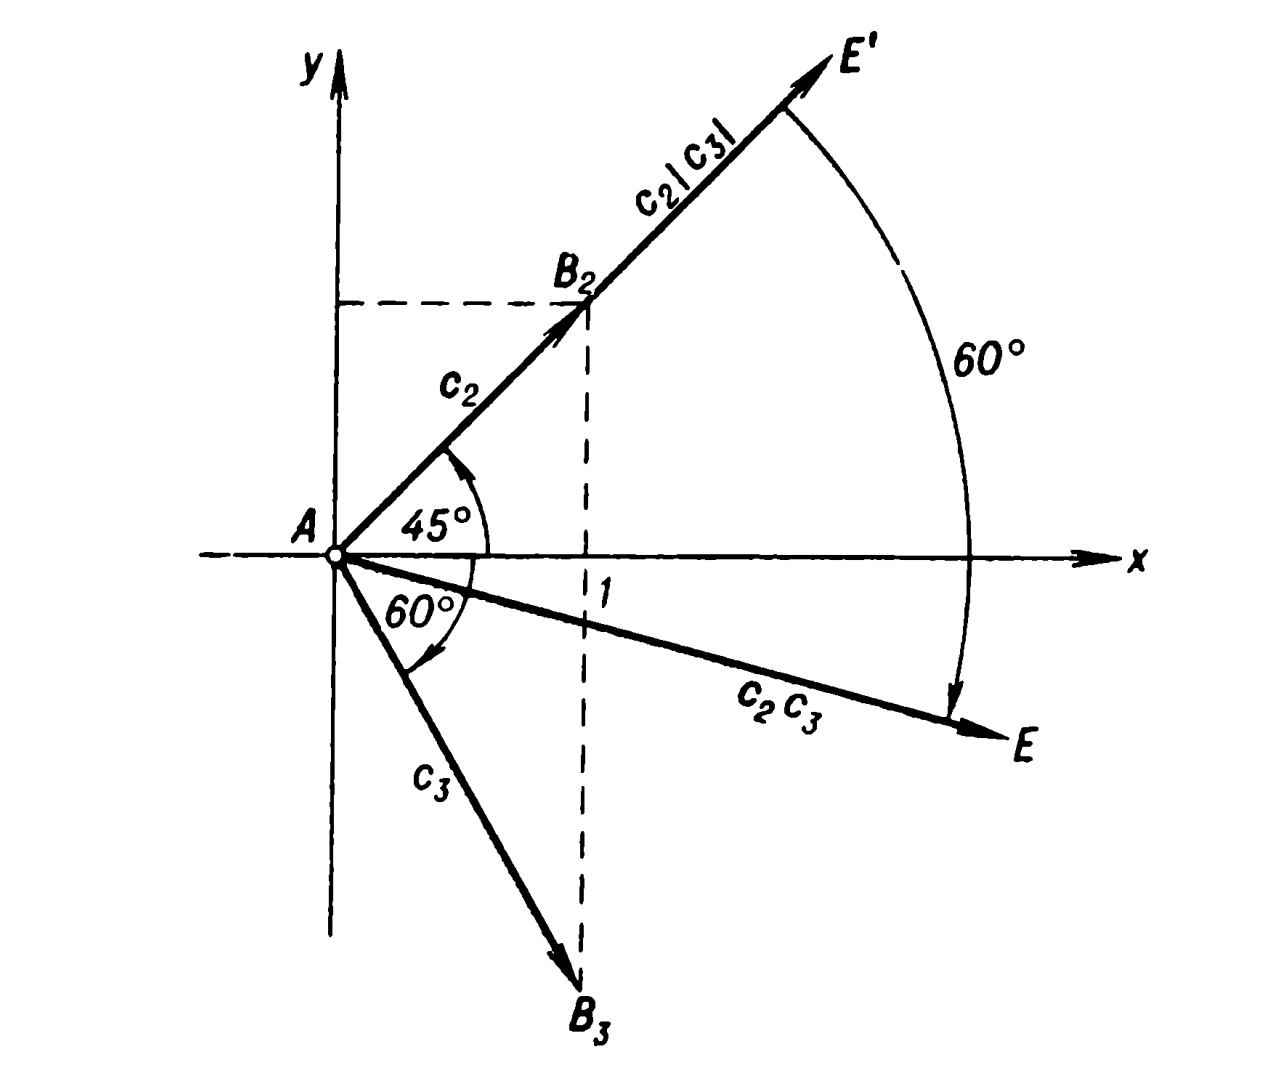
\includegraphics[width=.3\textwidth]{c1xc2} 
\end{center}
\end{figure}
%%%-----------------------------------------------------------------------------
Here is the multiplication of two vectors: $\langle 3,4\rangle$ (magnitude: 5) and $\langle 5,12\rangle$ (magnitude: 13) to produce the vector $\langle -33,56\rangle$ (magnitude: $5\times13=65$). Note: $\langle 33,56,65\rangle$ is a Pythagorian triple.
\begin{figure}[h]
\begin{center}
\caption{Another Geometric Interpretation of Complex Number Multiplication (Drawn to Scale using Geogebra)}
\label{fig:complexmult2}
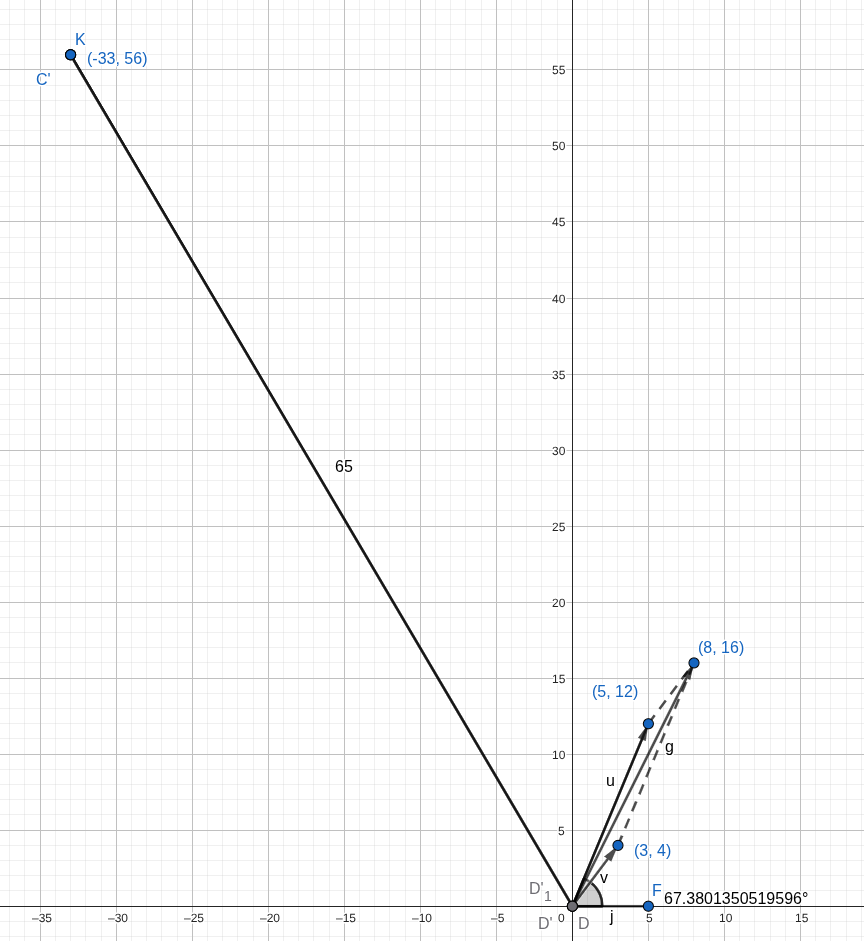
\includegraphics[width=.5\textwidth]{c1xc2-2} 
\end{center}
\end{figure}

\begin{problem}
\label{pr:affine}
If an operation for the ordered pairs of real numbers, denoted by $\boxdot$ again, is defined by
$$
\langle a,b\rangle\boxdot\langle c,d\rangle=\langle ac,ad+b\rangle
$$
, is it commutative? Is it associative?

Note: Looking strange is not necessarily a sign of being artificial or useless.
\end{problem}

\textbf{Solution}.

\begin{align*}
\langle a,b\rangle\boxdot\langle c,d\rangle=\langle ac,ad+b\rangle
\end{align*}
\begin{align*}
\langle c,d\rangle\boxdot\langle a,b\rangle=\langle ca,cb+d\rangle
\end{align*}

$\therefore \boxdot$ is not commutative in general; only commutative if $\frac{a-1}{b}=\frac{c-1}{d}$.
\begin{align*}
(\langle a,b\rangle\boxdot\langle c,d\rangle)\boxdot\langle m, n\rangle
&=\langle ac, ad+b\rangle\boxdot\langle m,n\rangle\\
&=\langle acm,acn+ad+b\rangle\\
\end{align*}
and
\begin{align*}
\langle a,b\rangle\boxdot(\langle c,d\rangle\boxdot\langle m, n\rangle)
&=\langle a,b\rangle\boxdot\langle cm,cn+d\rangle\\
&=\langle acm,acn+ad+b\rangle\\
\end{align*}

$\therefore \boxdot$ is associative.

\qedsymbol

\textbf{Halmos's Solution}.

Halmos describes an operation on functions: their composition. Consider two linear transformations of a real number (mapping of a real number onto another by a function $\mathbb {R}:\mathbb {R}$), $x$, where $a,b,c,d$ are known constants:
\begin{equation}
\begin{aligned}
f(x)=ax+b \\
g(x)=cx+d
\end{aligned}\label{eq:fg}
\end{equation}

Then, is composition of functions commutative? 

$$
(f\circ g)(x)=f(g(x))=f(cx+d)=a(cx+d)+b=acx+ad+b
$$
and
$$
(g\circ f)(x)=g(f(x))=g(ax+b)=c(ax+b)+d=acx+bc+d
$$

$\therefore (f\circ g)\ne(g\circ f)$.

However, consider the application of $(f\circ g)$ to $x$. It yields a result that is the same as the affine transformation of $x$ by $(ac, ad+b)$ which is itself an affine transformation ($\boxdot$) of $\langle a,b\rangle$ and $\langle c,d\rangle$. And since $(f\circ g\circ h)=f\circ(g\circ h)=(f\circ g)\circ h$\footnote{That is, function composition is associative (which can be easily proved)}, $\boxdot$ is also associative. 

\qedsymbol

\begin{problem}
\label{pr:matrixmult}
If an operation for the ordered quadruples of real numbers, denoted by $\boxdot$, is defined by
$$
\langle a,b,c,d\rangle\boxdot\langle a',b',c',d'\rangle=\langle aa'+bc',ab'+bd',ca'+dc',cb'+dd'\rangle
$$
, is it commutative? Is it associative?
\end{problem}

\textbf{Solution}.
Since the multiplication of real numbers is commutative ($aa'+bc'=a'a+c'b$, and so on), the \textit{matrix multiplication} defined here is commutative.

The visual symmetry in this operation feels useful in proving its associativity, although one should carry out the operation rigorously to believe that it is associative. That is left out here (we wouldn't say ``as an exercise to the reader!'').

It's easier to visualize this as a matrix:

\[
  \begin{pmatrix}
    a & b\\
    c & d\\
  \end{pmatrix}
  \begin{pmatrix}
    a' & b'\\
    c' & d'\\
  \end{pmatrix}
  =
  \begin{pmatrix}
    aa'+bc' & ab'+bd'\\
    ca'+dc' & cb'+dd'\\
  \end{pmatrix}
\]

\qedsymbol

How is Problem [\ref{pr:affine}] a ``special case'' of Problem [\ref{pr:matrixmult}]?

Consider
\[
  \begin{pmatrix}
    a & b\\
    0 & 1\\
  \end{pmatrix}
  \begin{pmatrix}
    a' & b'\\
    0 & 1\\
  \end{pmatrix}
  =
  \begin{pmatrix}
    aa' & ab'+b\\
    0 & 1\\
  \end{pmatrix}
\]

The first row of the result is the affine tranform of the first rows of the two matrices on the left-hand side. Halmos, being an algebraist, does not describe it so, however. 

Also, is Problem [\ref{pr:affine}] a ``special case'' of Problem [\ref{pr:complexmult}]?
Consider
\[
  \begin{pmatrix}
    a & b\\
    -b & a\\
  \end{pmatrix}
  \begin{pmatrix}
    c & d\\
    -d & c\\
  \end{pmatrix}
  =
  \begin{pmatrix}
    ac-bd & ad+bc\\
    -bc-ad &-bd+ac\\
  \end{pmatrix}
\]
I still don't understand how matrix multiplication is a "more general" case of vector multiplication or affine transform; it might become clear later.

\begin{problem}
\label{pr:modularmult}
Is multiplication modulo 6 commutative? Is it associative? What if 6 is replaced with 7: do the conclusions for 6 remain true or do they change?
\end{problem}

\textbf{Solution}.
I should refresh my number theory, but I will defer that for now. Let me attempt my solution from first principles.

Since multiplication of integers is commutative ($ab=ba \forall a,b\in\mathbb{N}$), $ab\mod 6=ba\mod 6$. This is true when modulus is any positive integer.

Consider four integers, $a,b,c,M\mid M\ne 0$. We call $M$ the modulus. Then, according to the division algorithm, following integers, $q_1,r_1,q_2,r_2,q_3,r_3\mid r_1,r_2,r_3<M$ exist:
\begin{equation}
\!
\begin{aligned}
a &= Mq_1+r_1\\
b &= Mq_2+r_2\\
c &= Mq_3+r_3\\
\end{aligned}\label{eq:abcM}
\end{equation}

Then, $abc\mod M=r_1r_2r_3\mod M$, because it follows from Equation [\ref{eq:abcM}] that $abc\equiv r_1r_2r_3 \pmod{M}$.

Since the product of the integers, $r_1r_2r_3$, is associative, the modular multiplication operation, $abc\mod M$, is also associative.

\qedsymbol

\textbf{Halmos's Solution}.

Halmos warns that the most tedius way of solving this problem (or perhaps any problem) is by exhaustion: Prove something by examining it for every possibility. Thus, if there are only 6 integers (0 through 5) for which to prove commutativity and associativity of the modulo-6 multiplication, we can exhaust all the 36 ordered pairs and 216 ordered triples respectively, and we are done. That is clearly boring.

He provides another way that is equivalent to my approach (that uses the versatile division algorithm). I like my solution better!

However, he concludes his solution thus that makes us curious:
\begin{reflection}
An important difference between the modular arithmetic of 6 and 7 will
become visible later, but for most of the theory they act the same way, and that
is true, in particular, as far as commutativity and associativity are concerned.
\end{reflection}


\begin{problem}
\label{pr:smallsets}
\end{problem}
Problem [\ref{pr:modularmult}] shows that interesting operations can exist on small sets. In that problem we were working with (binary) operations whose results were members of a set: $S=\{0,1,2,3,4,5\}$ and whose operands any natural numbers. Although ``small sets'' like $S$ may sometimes be misleading, they may be useful to develop insight.

Problem [\ref{pr:2a2b}] asked about a binary operation (on real numbers) that was commutative but not associative ($a\boxplus b=2a+2b$).

Remarkably, the modulo 3 multiplication and the modulo 3 addition on any two numbers from $\{0,1,2\}$ are commutative \textit{and} associative:

\begin{table}[h!]
\centering
\begin{tabular}{l|ccc}
$\times$&0&1&2\\
\hline
0&0&0&0\\
1&0&1&2\\
2&0&2&1\\
\end{tabular}
\quad\quad\quad
\begin{tabular}{l|ccc}
+&0&1&2\\
\hline
0&0&1&2\\
1&1&2&0\\
2&2&0&1\\
\end{tabular}
\caption{Two commutative and associative operations}
\label{tab:twoops}
\end{table}

Is there an operation in a set of three elements that is commutative but not associative?

\textbf{Solution}.

Halmos hasn't defined what an ``operation \textit{in} a set of three elements'' means. For instance, is the operation on two members of a three-member set that returns a result which is also a member of the same set, or must the result of that operation (like the modular multiplication of Problem [\ref{pr:modularmult}]) on any two natural numbers be a member of that set?\footnote{Later on, when I was discussing this with my son, he spontaneously said, ``That means the set is \emph{closed} under that operation''} From context, I assume the former and restate the problem:

Is there a binary operation that is commutative but not associative that takes (two) elements of a three-member set and whose result is also a member of that set?\footnote{More technically: Is there a commutative but not associative operation on a 3-element set which is closed under that operation?}

How do we start solving such a problem? It \emph{feels} insurmountable. As I write this, I have no clear idea. ``C’est la vie'', I guess! However, we can try gathering facts and look for any patterns, connections, etc. We need to find a set of three numbers, three nonnegative integers, $S=\{a,b,c\}$ and define an operation $\openbox$ such that
\begin{enumerate}
\item The result of $\square$ on any two elements of $S$--$a,b$ for instance--is an element of $S$,
\item $\square$ is commutative, i.e., $a\square b= b\square a$, and
\item $\square$ is \emph{not} associative, i.e.,$a\square(b\square c)\ne (a\square b)\square c$
\end{enumerate}

This is what abstract algebra comprises. It wants us to focus on operations on entities more than the entities themselves; \emph{operations} are of essence.

A weird operation \emph{occurred} to me. Let's call it an \emph{exclude} operation, denoted by $\openbox$. Here is its definition for operands from any set $S$ that has three or more elements:

\begin{definition}[Exclude operation:$\openbox$]
It accepts two operands and returns an element from $S$ \emph{excluding} its operands. When more than one element is available, it returns the smallest (which is guaranteed to be unique).
\end{definition}

\begin{table}[h!]
\centering
\begin{tabular}{l|ccc}
$\downarrow x\openbox y\rightarrow$&2&3&5\\
\hline
2&3&{\textcolor{red}5}&{\textcolor{blue}3}\\
3&{\textcolor{red}5}&2&{\textcolor{LimeGreen}2}\\
5&{\textcolor{blue}3}&{\textcolor{LimeGreen}2}&2\\
\end{tabular}
\caption{$\openbox$ is commutative for $S=\{2,3,5\}$}
\label{tab:exclude}
\end{table}

Table [\ref{tab:exclude}] shows that $\openbox$ is commutative.

What about its associativity? 

$2\openbox(3\openbox 5)=2\openbox 2=3$, but $(2\openbox 3)\openbox 5=5\openbox 5=2$.

Since the two are not the same, $\openbox$ is not associative.

\qedsymbol

\begin{reflection}
$\openbox$ satisfies the problem's requirements, but I don't know why it works; its discovery feels like art. It is hard to say if I could have found it by deduction alone. 
\end{reflection}
\textbf{Halmos's Solution}.

The answer may or may not be easy to guess, but once it's correctly guessed it's easy to prove. The answer is yes, and anyone who believes that and sets out to construct an example is bound to succeed.

Call the three elements for which multiplication is to be defined $\alpha,\beta,\gamma$; the problem is to construct a multiplication table that is commutative but not associative. (Note: It's not clear why he wants to construct a ``multiplication table''. Perhaps he means `matrix'. So, what does a commutative-but-not-associative matrix look like?)

Question: what does commutativity say about the table? Answer: symmetry about the principal diagonal (top left to bottom right). That is: if the entry in row $\alpha$ and column $\beta$ is, say, $\gamma$, then the entry in row $\beta$ and column $\alpha$ must also be $\gamma$.

How can associativity be avoided? How, for instance, can it be guaranteed that $ (\alpha\times\beta)\times\gamma\ne\alpha\times(\beta\times\gamma)$?
\begin{reflection}
I stumbled at this question. Predicting whether a binary operation is commutative given its `matrix' is not that difficult. You check if the element $M_{ab}$ equals $M_{ba}$ ($a$ and $b$ respectively denote the row number and the column number).

What is the `matrix-test' of an associative binary operation? Looking only at the matrix (like the one in Table [\ref{tab:exclude}]) of some unknown binary operation, can one tell if it is associative? How? The two operations in Table [\ref{tab:twoops}] are too disparate to discern a common pattern for an associative operation!

Since associativity requires three operands, should I visualize a cube? However, the set is closed under this operation, so just looking at the matrix should be enough. 

Should I consider cases?

Time to peek at Halmos's discussion further in a way suggested by R. L. Moore \cite{Moore1966} (one line or two at a time, while considering this act a failure of sorts)?
\end{reflection}

Possible approach: make $\alpha\times\beta=\gamma$ and $\beta\times\gamma=\alpha$; then the associative law will surely fail if $\gamma\times\gamma$ and $\alpha\times\alpha$ are different. That's easy enough to achieve and the following table is one way to do it:

\begin{table}[h!]
\centering
\begin{tabular}{l|ccc}
$\times$&$\alpha$&$\beta$&$\gamma$\\
\hline
$\alpha$&$\alpha$&$\gamma$&$\beta$\\
$\beta$&$\gamma$&$\beta$&$\alpha$\\
$\gamma$&$\beta$&$\alpha$&$\gamma$\\
\end{tabular}
\caption{A commutative and not associative operation}
\label{tab:comnotassoc}
\end{table}
Here, for what it's worth, is a verbal description of this multiplication: the product of two distinct factors is the third element of the set, and the product of any element with itself is that element again.

\begin{reflection}
This is close to my exclude operation, but Halmos's explanation uses a neat trick. By making $\alpha\times\alpha$ not agree with $\gamma\times\gamma$, we can avoid associativity. However, does it mean that the associativity test is not as obvious as the commutativity test?
\end{reflection}

The sum of $0$ and any real number $\alpha$ is $\alpha$ again; the product of $1$ and any real number $\alpha$ is $\alpha$ again: $1\times\alpha=\alpha\times 1=\alpha$. This phenomenon is described by saying that $0,1$ are \textbf{identity element}s (or zero elements, unit elements, or neutral elements) of addition and multiplication respectively. 

\begin{reflection}
Commutativity appears a prerequisite for identity. An operation that is not commutative does not have an identity element. For instance, $a\div 1=a\ne 1\div a$. Therefore, the $\div$ operation on reals does not have an identity element.
\end{reflection}

\begin{reflection}
Identity elements of operations remind me of ``fixed points'' of functions.
\end{reflection}

\begin{problem}
\label{pr:idelem}
Which of the operations
\begin{enumerate}
\item double addition (Problem [\ref{pr:2a2b}]),
\item half double addition (Problem [\ref{pr:2ab}]),
\item exponentiation (Problem [\ref{pr:atob}]),
\item complex multiplication (Problem [\ref{pr:complexmult}]),
\item multiplication of affine transformations (Problem [\ref{pr:affine}]),
\item matrix multiplication (Problem [\ref{pr:matrixmult}]), and
\item modular addition and multiplication (Problem [\ref{pr:modularmult}])
\end{enumerate}
have an identity element?
\end{problem}
\textbf{Solution}.

Based on the definition of identity element above, we designate the \emph{constant} $a\in\mathbb{C}$ an identity element of the operation $\openbox$, if for some $b\in\mathbb{C}$, $a\openbox b$ equals $b$. We consider the set of complex numbers which may be thought bigger than that of real numbers. We apply this in turn for each item above. Of course, the other rules of arithmetic (and complex numbers) hold. This scheme feels straightforward.
\begin{enumerate}
\item For the double addition $\openbox$, by definition,
$$
a\openbox b=2a+2b
$$
For the prospective \emph{identity element} $a$ of the $\openbox$ operation, $a\openbox b$ equals $b$.
$$
b=2a+2b
$$
$$
\therefore a=-\frac{b}{2}
$$

Since $b$ can be any real number, $a$ must be so too. It cannot be a constant. That is a contradiction. Therefore, this operation does not have an identity element.
\item For the half double addition $\openbox$, by definition,
$$
a\openbox b=2a+b
$$
For the prospective \emph{identity element} $a$ of the $\openbox$ operation, $a\openbox b$ equals $b$.
$$
b=2a+b
$$
$$
\therefore 2a=0\implies a=0
$$
Therefore, $0$ is the identity element of the half double addition. 
\begin{reflection}[Mistake Found on a Review]
I was on a plane. I wanted to review my LAPB work so far and I realized the mistake in the above argument.

Commutativity is a prerequisite for identity.

Therefore, if $i$ is the identity element of the half double addition, $a\openbox i=i\openbox a$. Also, $a\openbox i=2a+i=a$ gives us $i=-a$, whereas $i\openbox a=2i+a=a$ gives $i=0$. This is a contradiction.

So, I checked the answer. Halmos reasons how we do. He says:
\begin{sidebar}[Right-Left Identity]
Half double addition has no \textbf{right identity element} but it does have a \textbf{left identity element}.
\end{sidebar}
More terminology!
\end{reflection}

\item For exponentiation, $b^a=b=b^1\implies a=1$. Therefore, $1$ is the identity element of exponentiation (like multiplication).

\begin{reflection}[Another Oddity]
Commutativity is a prerequisite for identity element: $a^i=i^a=a$. $a^i=a\implies i=1$, whereas $i^a=a$ does not result in a constant value for $i$. This is the opposite (or backward as Halmos calls it) case. 
\end{reflection}

\item Complex multiplication is a bit more complicated. We are seeking a \emph{complex number} $c_1$, which is a pair of real numbers, $(a,b)$, such that $c_1\times c_2$ equals $c_2$, where $c_2$ is a pair of real numbers, $(c,d)$.

By definition,
$$
(a,b)\times(c,d)=(ac-bd,ad+bc)=(c,d)
$$
\begin{equation}
\label{eq:c1}
ac-bd=c
\end{equation}
and
\begin{equation}
\label{eq:c2}
ad+bc=d
\end{equation}

Equation [\ref{eq:c1}]$\times c+$Equation [\ref{eq:c2}]$\times d$ yields

$$
a(c^2+d^2)=c^2+d^2
$$
and, since $c^2+d^2\ne 0$, $a=1$. Then, from equation [\ref{eq:c1}], $bd=0\implies b=0$.

Therefore, the \emph{complex number} $(1,0)$ is the identity element of complex multiplication. Indeed, $(1,0)\times(c,d)=(1\times c-0\times d,1\times d+0\times c)=(c,d)$.

\item\label{item:affine} Affine transformation of two pairs of real numbers, $\langle a,b\rangle$ and $\langle c,d\rangle$, is the pair $\langle ac,ad+b\rangle$ for which to be the same as $\langle c,d\rangle$, $\langle a,b\rangle$ must be $\langle 1,0\rangle$, which is the identity element of affine transformation multiplication.
\item\label{item:matmultidelem} It's not hard to see that the matrix
\[
  \begin{pmatrix}
    1 & 0\\
    0 & 1\\
  \end{pmatrix}
\] 
is the identity element of matrix multiplication.
\item Since $0$ is the identity element of addition, it is also the identity element of modular addition. Similarly, since $1$ is the identity element of multiplication, it is also the identity element of modular multiplication. 
\end{enumerate}

\qedsymbol

A tradition followed in this book is that multiplication is a more general operation than addition. However, we should bear in mind addition is always commutative, multiplication may not be (e.g., matrix multiplication). 

\begin{reflection}
If addition is a ``special case'' of multiplication, exactly what makes the former commutative and latter not always so?

I hope that becomes clear in the due course \dots.
\end{reflection}

A mini-theorem now.
\begin{mini-theorem}
An operation (a binary operation) can have at most one identity element.
\end{mini-theorem}
\begin{proof}
We prove by contradiction that if an identity element exists for a given operation, it must be unique. Let there be two distinct identity elements, $e$ and $e'$. Thus, we assume that $e\ne e'$.

By definition, identity element(s) are commutative: $a\openbox b=b\openbox a$. If we use $a=e$ and $b=e'$, we get $e\openbox e'=e'\openbox e$ and it follows that $e=e'$. A contradiction. Therefore, $\openbox$ can have at most one identity element.
\end{proof}

Associativity and identity element of an operation are closely related to another interesting property of an operation defined below.

\begin{definition}[$*$ Inverse of $x$] 
Suppose that a binary operation $*$ has an identity element $\varepsilon$ such that $\varepsilon*x=x*\varepsilon=x\forall x$. Then, an element $\beta$ is called the ``$*$ inverse'' of $x$ if 
$$
x*\beta=\beta*x=\varepsilon
$$
\label{def:*-inverse}
\end{definition}

Note that an operation $*$ can have an identity element, but not every element in the set to which its operands belong has a $*$ inverse.
\begin{example} For the set $\mathbb{R}$ of real numbers, the multiplication operation $\times$ has an identity element $\varepsilon=1$; but $0\in\mathbb{R}$ does not have a $\times$ inverse. There is no $\beta\in\mathbb{R}$ such that $0\times\beta=1$. In other words, $0$ is the only real number that fails to be \emph{invertible} under $\times$. 
\end{example}
\begin{example} For the set $\mathbb{R}$ of real numbers, the addition operation $+$ has an identity element $\varepsilon=0$. Every real number has a $+$ inverse.
\end{example}
\begin{mini-theorem}
If $*$ is an associative operation, then any element it operates on has at most one inverse.
\end{mini-theorem}
\begin{proof}
Left as an exercise.
\end{proof}

\begin{problem}
\label{pr:complexinv}
For complex multiplication (defined in Problem [\ref{pr:complexmult}]), which ordered pairs $\langle a,b\rangle$ are invertible? Is there an explicit formula for the inverses of the ones that are?
\end{problem}

\textbf{Solution}.

\begin{reflection}
This felt like a straightforward problem. By extension of the real multiplication, perhaps $\langle 0,0\rangle$ is the only complex number whose (complex) inverse does not exist.
\end{reflection}

We want to learn something about the \emph{complex inverse} of $\langle a,b\rangle$. Let $\langle c,d\rangle$ be that inverse. Then, by definition,

$$
\langle a,b\rangle\cdot\langle c,d\rangle=\varepsilon=\langle 1,0\rangle
$$

It follows that 
$$
\langle ac-bd,ad+bc\rangle=\langle1,0\rangle
$$
And
\begin{equation}
\!
\begin{aligned}
ac-bd=1 \\
ad+bc=0
\end{aligned}\label{eq:complexinv1}
\end{equation}
Then after eliminating $d$, we get
\begin{equation}
\!
\begin{aligned}
c=\frac{a}{a^2+b^2} \\
d=\frac{-b}{a^2+b^2}
\end{aligned}\label{eq:complexinvformula}
\end{equation}

Therefore, if ${a^2+b^2}\ne 0$, a complex inverse of $\langle a,b\rangle$ exists. We can use the formula in equation [\ref{eq:complexinvformula}] to calculate the $\cdot$ inverse of any complex number. The only exception is the complex number $\langle 0,0\rangle$ whose $\cdot$ inverse does not exist because $a^2+b^2=0$.

\qedsymbol

\begin{problem}
\label{pr:affineinv}
For the multiplication of affine transformations (defined in Problem [\ref{pr:affine}]), which ordered pairs $\langle a,b\rangle$ are invertible? Is there an explicit formula for the inverses of the ones that are?
\end{problem}

\textbf{Solution}.
\begin{reflection}
This feels like an \emph{exercise}. Should I look at it like what P\'{o}lya said (It is better to solve a problem 5 different ways rather than solving five different problems the same way)?
\end{reflection}
Proceeding as above and using $\langle 1,0\rangle$ as the identity element of affine transformations (Cf. item [\ref{item:affine}]), it follows that

$$
\langle ac,ad+b\rangle=\langle 1,0\rangle
$$
$$
\therefore c=\frac{1}{a}, d=-\frac{b}{a}
$$

The affine inverse of $\langle a,b\rangle$ is $\langle\frac{1}{a},-\frac{b}{a}\rangle$ which exists if $a\ne 0$.

\textbf{Halmos's Solution}.

Halmos proceeds along similar lines. However, he draws our attention to the fact that affine transformation is not commutative! 

\begin{reflection}
That's strange! Commutativity is a requirement for the definition of the identity element of an operation. If the multiplication of affine pairs is not commutative, how can its inverse (even the so-called `right' inverse) be defined?

We have covered a lot of ground. Commutativity, associativity, identity element, inverse. The concepts are of course related, but I feel wary. For the uniqueness of identity element of an operation and that of its ``operation inverse'', that operation needs to be commutative, by definition (Cf. Definition [\ref{def:*-inverse}]). And yet, we are analyzing an operation (e.g., affine multiplication, matrix multiplication) on a pair of real numbers that is not commutative. Isn't that discrepancy troublesome?  

Consider two `numbers', $e_1,e_2$, which are elements of a set $S$ (e.g., $S=\{\langle x,y\rangle\mid x,y\in\mathbb{R}\}$), and an operation $\openbox$ that operates on two elements of $S$ and produces a result that is also an element of $S$. 

Let $e_1\openbox e_2=e_3$ and $e_3\openbox e_4=e_1$ again. Then, $e_4$ is the ``$\openbox$ inverse'' of $e_2$ (because it `reverses' the effect of $e_2$ on $e_1$). If there is no such element $e_4$, then the element $e_2$ is not invertible under $\openbox$.

Would that definition of inverse be less troublesome? Here we do not make commutativity a requirement and we do not yet refer to the identity element of an operation.

Perhaps that is what one-sided inverse means. It may then turn out that $e_2\openbox e_4$ equals $e_i$, the identity element for the operation $\openbox$.
\end{reflection}

\begin{problem}
\label{pr:matrixinv}
Which of the $2\times2$ matrices 
$$
  \begin{pmatrix}
    a & b\\
    c & d\\
  \end{pmatrix}
$$
(for which multiplication was defined in Problem [\ref{pr:matrixmult}]), are invertible? Is there an explicit formula for the inverses of the ones that are?
\end{problem}

\textbf{Solution}.
Invertible matrices\dots\tbd{Work out invertible matrices}

Numbers can be added, subtracted, multiplied, and (with one infamous exception) divided. 

\emph{Linear algebra is about concepts called scalars and vectors.}

Scalars are usually numbers; to understand linear algebra it is necessary first of all to understand numbers, and, in particular, it is necessary to understand what it means to add and subtract them. The general concept that lies at the heart of such an understanding is that of \textbf{Abelian groups}.

\begin{definition}[Abelian Group]
It is a set $\mathbb{G}$ with an operation of `addition' ($+$) defined \emph{in} it (so that whenever $x,y\in\mathbb{G}$, $x+y\in\mathbb{G}$). The addition operation satisfies four conditions: commutativity, associativity, the existence of a zero, and, corresponding to each element, the existence of its negative (also called its $+$ inverse).\footnote{Clarify: Are the zero of the operation and every element's negative unique?}
\end{definition}



\begin{example}
$(\mathbb{Z},+)$, the set of integers along with the addition operation, is an abelian group. $\mathbb{Z}$ is closed under $+$. $+$ is commutative. $+$ is associative. The element $0\in\mathbb{Z}$ is the zero of $+$ and every $x\in\mathbb{Z}$ has a corresponding negative (also called the \emph{additive inverse}), viz., $-x\in\mathbb{Z}$.
\end{example}

Almost exactly the same statements can be made about every abelian group; the only differences are terminological (the words `integer' and `addition' may be replaced by others) and notational (the symbols $0$ and $+$ may be replaced by others).


`Abelian' group implies `commutative' group. If the $+$ operation does \emph{not} satisfy the commutativity condition, then it is simply a `group' (and not an Abelian group) or a non-commutative group. The study of linear algebra includes a deeper study of commutative and non-commutative groups.

\begin{problem}
\label{pr:abelian}
%\renewcommand{\theenumi}{\alph{enumi}}
\begin{enumerate}
\item If a new operation $*$ is defined in the set $\mathbb R_{> 0}$ (the set of positive real numbers) by
$$ 
x*y=min(x,y)
$$
, does $\mathbb R_{>0}$ become an abelian group?
\item If a new operation $*$ is defined in the set $S=\{1,2,3,4,5\}$ by
$$
x*y=max(x,y)
$$
, does $S$ become an abelian group?
\item\label{item:xyyx0p} If $x$ and $y$ are elements of an abelian group such that $x+y=y$, does it follow that $x = 0$?
\end{enumerate}

\end{problem}

\textbf{Solution}.
\begin{enumerate}
\item The $min$ operation is defined on $\mathbb R_{>0}$ as follows:
$$
*: min(x,y)=
\begin{cases}
x\quad\text{if}\quad x<y\\
y\quad \text{otherwise}
\end{cases}
$$

The set $\mathbb R_{>0}$ is closed under the operation $*:min(x,y)$ because it returns one of its operands both of which are in the set.

Since, by definition, the operation $*$ chooses the smaller of its operands \emph{regardless of their order}, the order does not affect its outcome: $min(x,y)=min(y,x)$. Therefore, the operation is commutative. Extending the same argument to three (or more) operands we deduce that the operation is associative. Associativity can also be proved exhaustively by considering all the $3!\cdot 2^2=24$ possible cases: $\{\langle x<y<z\rangle,\langle x<z<y\rangle,\dots,\langle z\nless y \nless x\rangle\}$. We can also use the transitivity of the relationship `<' between two positive real numbers.

We note that the set $\mathbb R_{>0}$ is an infinite set and $0\not\in\mathbb R_{>0}$. The element $e_i$ of $\mathbb R_{>0}$ that is greater than its all other elements is the identity (zero) element of this operation, $*$, such that $min(x, e_i)=x\forall x\in\mathbb R_{>0}$. However, there is no such element in this set and therefore the operation does not have a zero. Consequently, $(\mathbb R_{>0},*)$ is not a group (and hence not an abelian group).

Even so, does $*$ have the property such that every element of $\mathbb R_{>0}$ has a corresponding `negative' element that is also a member of $\mathbb R_{>0}$?

If $(a*b)*d=a$, then $d$ is the `negative' (denoted by $\circledast$) of $*$.

We can see that if $a\leq b$, then $a*b=a$ and $(a*b)*b=a*b=a$, implying $d=\circledast b=b$, i.e. $b$ is its own negative. However, if $a>b$, then $(a*b)*b=b*b=b\leq a$ implying that $b$ is \emph{not} its own negative. Therefore, the negative does not exist.\footnote{A more rigorous argument can be made by introducing an element $\epsilon>0$}
\item The $max$ operation is defined on $S=\{1,2,3,4,5\}$ as follows:

$$
*: max(x,y)=
\begin{cases}
x\quad\text{if}\quad x>y\\
y\quad \text{otherwise}
\end{cases}
$$
The set $S$ is closed under the operation $*:max(x,y)$ because it returns one of its operands both of which are in the set.

Since, by definition, the operation $*$ chooses the greater of its operands \emph{regardless of their order}, the order does not affect its outcome: $max(x,y)=max(y,x)$. Therefore, the operation is commutative. Extending the same argument to three (or more) operands we deduce that the operation is associative. Associativity can also be proved exhaustively by considering all the $3!\cdot 2^2=24$ possible cases: $\{\langle x>y>z\rangle,\langle x>z>y\rangle,\dots,\langle z\ngtr y \ngtr x\rangle\}$. We can also use the transitivity of the relationship `>' between two positive integers numbers less than or equal to 5.

Curiously, 1 is the element of $S$ such that $x*1=x\forall x\in S$. Therefore, $1$ is the zero of this operation.

However, only 1 has a negative, namely, itself, but none of $2,3,4$, and 5 has a negative. Therefore $(S,*)$ is not a group (and not an abelian group).

\item\label{item:xyyx0s} No! It does not.

\begin{remark}
Halmos: It (this item) is easy, but it's here because it is useful and, incidentally, because it shows how the defining axioms of groups can be useful. What was proved in Problem [\ref{pr:idelem}] is that if an element acts the way 0 does for every element, then it must be 0; this part here asks about elements that act the way 0 does for only one element.
\end{remark}
(I read Halmos's remark above to clarify that the problem states that there is one specific number $y\in\mathbb{G}: x+y=y$ and asks if $x$ qualifies as the zero of $+$).

Consider $\mathbb{G}=(\mathbb Z,\times)$. We know that the set of integers and the addition operation is an abelian group. Consider $y=0$. Then $x=0$ is a number such that $x\times y=0\times 0=y$. This does not, however, make $x=0$ the zero of the $\times$ operation on $\mathbb Z$, there is at least one other number $y=1$ for which $x\times y=0\times 1=0\ne y$.

My answer shows one exception. However, Halmos asserts $x=0$ in his answer: Add $-y$ to both the sides and we get $x=0$. (But the inverse ($-y$) may not always exist for all the elements.)
\end{enumerate}

\begin{remark}
Group theory is deep and pervasive: no part of mathematics is free of its influence. At the beginning of linear algebra not much of it is needed, but even here it is a big help to be able to recognize a group when one enters the room.
\end{remark}
%%% Things to do
\begin{problem}
\label{pr:groupexs}
A few group problems:
\begin{enumerate}
\item Is the set of all affine transformations $x_i\mapsto ax_i+b$ (with the operation of functional composition) a group?
\item What about the set of all $2\times 2$ matrices (of real numbers)
$$
  \begin{pmatrix}
    a & b\\
    c & d\\
  \end{pmatrix}
$$ (with matrix multiplication)?
\item Is the set of nonzero integers modulo 6 (that is: the set of numbers 1,2,3,4,5) a group with respect to multiplication modulo 6?
\item  What if 6 is replaced by 7: does the conclusion remain true or does it change?
\end{enumerate}
\end{problem}
\textbf{Solution}. 

\begin{enumerate}

\item We denote the set of all affine transformations by $A_{ab}$ and the function composition operation by $\circ$. Then for the given constants, $a,b\in\mathbb{R}$, we have:
\begin{equation}
\begin{aligned}
\mathbb{R}&=\{\dots,x_1,x_2,x_3,a,b\dots\}\\
A_{ab}&=\{\dots,ax_1+b,ax_2+b,ax_3+b,a\cdot a+b,ab+b,\dots\}\\
\mathbb{G}&=(A_{ab},\circ)
\end{aligned}\label{eq:affinegroup}
\end{equation}

Is $\mathbb{G}$ a group?

\begin{reflection}
Is my reformulation of the problem correct? If yes, then this problem is unclear because I don't understand how ${A_{ab}}$ is closed under function composition operation. If not, then I am looking for a correct reformulation.

I read ahead: hint(s) and the solution, but they are not satisfactory; unfortunately, they don't clarify my confusion. 

What to do in such situations? Ask your friends (who are too busy to solve my problems!), or resort to a reliable online community like \texttt{math.stackexchange}? \textcolor{red} {Both choices are time-consuming to the extent of being impractical (remember Paul Garrett's thoughts on reading a math book \cite{PaulGarrettMathSE} at least in this case. I am going to skip this problem. I wish Halmos were clearer!}
\end{reflection}

\item We denote the set of all $2\times 2$ matrices of real numbers by $M_2$ and the matrix multiplication operation by $\times$. Then we have:
\begin{equation}
\begin{aligned}
M_2&=\left\{
  \begin{pmatrix}
    a_i & b_i\\
    c_i & d_i\\
  \end{pmatrix}
  \mid
  i\in\mathbb{Z}, a_i,b_i,c_i,d_i\in\mathbb{R}
\right\}\\
\mathbb{G}&=(M_2,\times)
\end{aligned}\label{eq:mmultgrp}
\end{equation}

Is $\mathbb{G}$ a group?

\textbf{Closure}: The set $M_2$ is closed under matrix multiplication because the set $\mathbb{R}$ of real numbers is closed under multiplication: A matrix produced by multiplying any two matrices in $M_2$ is in $M_2$. 

\textbf{Associativity}: For the sake of completeness, let
\begin{equation}
\begin{aligned}
  \mathbb{P}=\begin{pmatrix}
    a_i & b_i\\
    c_i & d_i\\
  \end{pmatrix}
  \times
  \begin{pmatrix}
    a_j & b_j\\
    c_j & d_j\\
  \end{pmatrix}
  =
  \begin{pmatrix}
    a_ia_j+b_ic_j & a_ib_j+b_id_j \\
    c_ia_j+d_ic_j & c_ib_j+d_id_j\\
  \end{pmatrix}
\end{aligned}\label{eq:exmaxmult}
\end{equation}
And
\begin{equation}
\begin{aligned}
  \mathbb{P}\times\begin{pmatrix}
    a_k & b_k\\
    c_k & d_k\\
  \end{pmatrix}
  =
  \begin{pmatrix}
  \dots \text{omitted}
  \end{pmatrix}
\end{aligned}\label{eq:assocp}
\end{equation}

It will be found that the associativity of matrix multiplication (I can easily write a computer program to generate the product) follows from the associativity of multiplication of real numbers: $abc=a(bc)=(ab)c$.

\textbf{Existence of the Zero}: We have already seen (Item [\ref{item:matmultidelem}]) that the zero of the matrix multiplication is the identity matrix 
$$
  \mathbb{I}=\begin{pmatrix}
    1 & 0\\
    0 & 1\\
  \end{pmatrix}
$$

$M\times\mathbb{I}=M\forall M\in M_2$.

\textbf{Existence of $\times$ Inverse}: Consider $M,N\in M_2$ such that $M\times N=R$. By definition of $M_2$, $R\in M_2$. 

Let's see if $\exists S\in M_2\mid R\times S=m$. Since $S$ \emph{reverses} the `$\times$' effect of $N$ on $M$, we say $S$ is the $\times$ inverse of $N$.

$\therefore (\text{from associativity})\; M\times N\times S=M\times(N\times S)=M$.

But, we also know from the identity element, that $M\times\mathbb{I}=M\implies N\times S=\mathbb{I}$.

Let 
$$
  M=\begin{pmatrix}
    a & b\\
    c & d\\
  \end{pmatrix},
  N=\begin{pmatrix}
    p & q\\
    r & s\\
  \end{pmatrix}
$$
We get the following linear equations from the matrix equation $N\times S=\mathbb{I}$.
\begin{equation}
\begin{aligned}
ap+br &= 1\\
aq+bs &= 0\\
cp+dr &= 0\\
cq+ds &= 1
\end{aligned}\label{eq:4eq4var}
\end{equation}

Linear algebra is supposed to solve such problems readily (finding $p,q,r,s$ in terms of $a,b,c,d$), but that's the technique we are learning. So, we should resort to the familiar technique of elimination. Grouping the first and the third together (and the second and the fourth together), we can evaluate $p,r$ (and $q,s$) easily. Here is a symmetric-looking solution of the system in equation [\ref{eq:4eq4var}]:
\begin{equation}
\begin{aligned}
p &= \frac{d}{ad-bc} \\
q &= \frac{-b}{ad-bc} \\
r &= \frac{-c}{ad-bc} \\
s &= \frac{a}{ad-bc}
\end{aligned}\label{eq:4eq4varsol}
\end{equation}

Therefore, as long as $ad-bc\ne0$, the inverse of the matrix 

$$
  M=\begin{pmatrix}
    a & b\\
    c & d\\
  \end{pmatrix}
$$
is the matrix
$$
  N=\begin{pmatrix}
    \frac{d}{ad-bc} & \frac{-b}{ad-bc}\\
    \frac{-c}{ad-bc} & \frac{a}{ad-bc}\\
  \end{pmatrix}
$$

By definition, $N\in M_2$.

Therefore, we say that the set of all \emph{invertible} $2\times 2$ matrices, with the multiplication operation, is a group.

\item Let 
$$
\mathbb{S}=\{1,2,3,4,5\}
$$
$$
\mathbb{G}=(\mathbb{S},\times_6), \text{where} \times_6 \text{is the modulo 6 multiplication operation}
$$

Then, $\mathbb{G}$ is not a group because it fails the closure property: $3\times_62=3\times2\bmod 6=6\bmod 6=0\not\in\mathbb{S}$.

\item\label{item:multmod7} Let 
$$
\mathbb{S}=\{1,2,3,4,5,6\}
$$
$$
\mathbb{G}=(\mathbb{S},\times_7), \text{where} \times_7 \text{is the modulo 7 multiplication operation}
$$

We expect nothing to change just by changing the \emph{modulus} from 6 to 7. One should, however, expect surprises from prime numbers (7 is one); prime numbers don't cease to amaze us. 

Are there two elements $a,b\in\mathbb{S}$ such that $a\times b \mod 7=0$? Or, equivalently, $7\mid a\times b$? 

We can \emph{exhaustively} prove that there are no such elements in $\mathbb{S}$. But here is a more delightful proof\footnote{My son gave this proof over a casual conversation; credit is due to him}:

We use contradiction. Let there be $a,b\in\mathbb{S}$ such that $a\times b=7m \text{ where } m\in\mathbb{N}$. 

From the Fundamental Theorem of Arithmetic, either $a<7,b<7,m$ are prime, or have the following (prime) factors (assuming $a$ has $p$, $b$ has $q$, and $m$ has $r$ prime factors):
$$
a=a_1\times a_2\times\dots\times a_p
$$
$$
b=b_1\times b_2\times\dots\times b_q
$$
$$
m=m_1\times m_2\times\dots\times m_r
$$

It follows that 

\begin{equation}\label{eq:ab=7m}
a_1\times a_2\times\dots\times a_p\times b_1\times b_2\times\dots\times b_q=7\times m_1\times m_2\times\dots\times m_r
\end{equation}

Since all the numbers in that expression are prime, it follows that one of the $a_i$'s or $b_i$'s is 7. Therefore, either $7\mid a$ or $7\mid b$. However, that is a contradiction because $a<7,b<7$.

If $a,b$ are prime, then also the equation [\ref{eq:ab=7m}] leads to a contradiction because the left hand side has no $7$ in a multiplication of integers but the right hand side does.
\qedsymbol

We can extend the proof to any prime number modulus. 

\textbf{Closure}: This leads us to deduce that $a\times_7 b=a\times b\mod 7=c\in\mathbb{S}$. Thus, the closure property is now satisfied. 

\textbf{Associativity}: Since $\times$ is associative, $\times_7$ is so too.\footnote{Do we need a stronger proof (e.g., using the division algorithm and theorems of modular arithmetic)?}

\textbf{Existence of the Zero}: $1\in\mathbb{S}$ is the zero of $\times_7$ because $x\times_7 1=x\forall x\in\mathbb{S}$. 

\textbf{Existence of $\times_7$ Inverse}: $1\in\mathbb{S}$ has such an inverse, namely, $1$ itself: $(x\times_7 1)\times_7 1=x\;\forall x\in\mathbb{S}$. Working along further, we find the inverse of each element of $\mathbb{S}$ in Table [\ref{tab:mod7inv}]. 


\begin{table}[h!]
\centering
\begin{tabular}{l|c}
$x\in\mathbb{S}$&$x^{-1}\in\mathbb{S}$\\
\hline
1&1\\
2&4\\
3&5\\
4&2\\
5&3\\
6&6
\end{tabular}
\caption{The $\times_7$ Inverse of Each Element of $\mathbb{S}$}
\label{tab:mod7inv}
\end{table}

\begin{reflection}
This surprised me. I went back and forth on deciding whether every element of $\mathbb{S}$ has a $\times_7$ inverse, especially when I erroneously calculated a few modulo 7 multiplications in my head! 

I then meticulously worked out modulo 7 multiplication tables that revealed this surprise.

Naturally I wondered: ``Can this be generalized\footnote{tbd: Prove or disprove} for any \emph{prime} modulus?''

The generalized problem could be: Is the set $\mathbb{S}=\{1,2,3,\dots,p-1\mid p\;\text{is prime}\}$, with the multiplication modulo $p$ operation a group? If yes, what is the multiplication modulo $p$ inverse of every $x\in\mathbb{S}$?

I then conjectured\footnote{I am glad that I did!} that the following holds $\forall x, x_i\in\mathbb{S}$, where $x,x_i$ are multiplication modulo $p$ inverses of each other: 
$$
x\times x_i\equiv 1 \pmod p
$$

\end{reflection}

\textbf{Halmos's Solution}. It is beautiful. Halmos asks illuminating questions along the way: 

If $\alpha$ is any one of the numbers $1,2,3,4,5,6$, what can be said about the numbers
$$
\alpha\times1,
\alpha\times2,
\alpha\times3,
\alpha\times4,
\alpha\times5,
\alpha\times6
$$
(multiplication modulo $7$)?

First answer: none of them is $0 \mod 7$. (Why? This is important, and it requires a moment's thought.\footnote{We proved it above (Item [\ref{item:multmod7}])}

Second (as a consequence of the first): they are all different. Why?

\begin{reflection}
I will attempt to prove it. First, let me state it in a general form.

Let $\mathbb{S}=\{1,2,3,\dots,p-1\}\;\text{where $p$ is a prime number}$. Let $\alpha$ be an element of $\mathbb{S}$. Prove that $\alpha\times i\pmod p\ne\alpha\times j\pmod p\;\text{where}\;i,j\in\mathbb{S}, i\ne j$.

\begin{proof}
Given:
$$
\alpha,i,j<p
$$
From Item [\ref{item:multmod7}], 
$$
$$
\begin{equation}
\begin{aligned}
\alpha\times i\pmod p&\ne 0\quad\forall i\in\mathbb{S}\\
\end{aligned}\label{eq:aimodp}
\end{equation}
Without the loss of generality, we let $i<j$.

We use contradiction. 

Assume the contrary, i.e., $\alpha\times i\pmod p=\alpha\times j\pmod p$

From the division algorithm it follows that $\exists q_1,q_2,r_1,r_2\in\mathbb{N}$ such that
\begin{equation}
\begin{aligned}
\alpha\times i=q_1\times p+r_1\\
\alpha\times j=q_2\times p+r_2
\end{aligned}\label{eq:aimodpdivalgo}
\end{equation}

However, $r_1=\alpha\times i\pmod p$, and $r_2=\alpha\times j\pmod p$, and we assumed them to be equal.

Then, from equation [\ref{eq:aimodpdivalgo}] it follows that

\begin{equation}
\begin{aligned}
\alpha\times(j-i)=p\times(q_2-q_1)\implies\exists k=j-i\in\mathbb{S}\mid\alpha\times k=0\pmod p
\end{aligned}\label{eq:aimodpraa}
\end{equation}
Equation [\ref{eq:aimodpraa}] contradicts with equation [\ref{eq:aimodp}]. This contradiction arises due to our (faulty) assumption that $r_1$ equals $r_2$. Therefore, $r_1\ne r_2\implies\alpha\times i\pmod p\ne\alpha\times j\pmod p$.
\end{proof}
\end{reflection}

Third (as a consequence of the second): except possibly for the order in which they appear, they are the same as the numbers $1,2,3,4,5,6$, and therefore, in particular, one of them is 1. That is: for each number $\alpha$ there is a number $\beta$ such that $\alpha\times\beta=1$: this is exactly the assertion that every $\alpha$ has a multiplicative inverse. 

Conclusion: the nonzero integers modulo 7 form a multiplicative group.

\end{enumerate}

\hrulefill

Here is another sample of Halmos's writing genius. He introduces the independence of group axioms thus:
\begin{sidebar}
A group is a set with an operation that has three good properties, namely associativity, the existence of an identity element, and the existence of inverses.

Are those properties totally independent of one another, or is it the case that some of them imply some of the others? So, for example, must an associative operation always have an identity element? The answer is no, and that negative answer is one of the first things that most children learn about arithmetic. We all learn early in life that we can add two positive integers and get a third one, and we quickly recognize that that third one is definitely different from both of the numbers that we started with--the discovery of zero came to humanity long after the discovery of addition, and it comes similarly late to each one of us. 

Very well then, if we have an associative operation that does possess an identity element, does it follow that every element has an inverse?

The negative answer to that question reaches most of us not long after our first arithmetic disappointment (see the solution to this Problem Item [\ref{item:xyyx0p}]): in the set $\{0,1,2,3,\dots\}$ we can add just fine, and 0 is an identity element for addition, but $+$ inverses are hard to come by--subtraction cannot always be done. After these superficial comments there is really only one sensible question left to ask.
\end{sidebar}

\begin{problem}
Can there exist a non associative operation with an identity element, such that every element has an inverse?
\end{problem}
\textbf{Solution.}

\begin{reflection}
I started without much clue, but it felt like I was getting somewhere. I hope I find a valid proof\dots
\end{reflection}
\begin{proof}
We have a set $\mathbb{S}=\{a,b,c,\dots,i,\dots,a_i,b_i,c_i\dots\}$ and an operation $\openbox$ such that $x\openbox x_i=x_i\openbox x=i\quad\forall x\in\mathbb{S}$. $i$ is the identity element.

We will use contradiction. Let us assume that $\openbox$ is not associative. Consider the operation $x\openbox x_i\openbox x$. Because of our assumption, $(x\openbox x_i)\openbox x\ne x\openbox(x_i\openbox x)$.

However,

$(x\openbox x_i)\openbox x=i\openbox x=x$,

and

$x\openbox(x_i\openbox x)=x\openbox i=x$.


This is a contradiction. Therefore, our assumption is incorrect and the operation must be associative. (Note: The definition of identity element requires commutativity.)
\end{proof}
\bogusproof

\begin{reflection}
Oh! Bogus proof.

I committed a blunder! I proved (!) that associativity is a requirement by only taking certain elements. It did not occur to me that the case I analyzed is not a general case. I did not consider the result of a general case like, for example, $a\openbox b_i\openbox c$. 

One can improve at math only slowly. Some people can of course do it faster than you, but you must do it slowly. This problem taught me that lesson. I thought ``I was in \emph{flow}'' and could not realize my own folly. Perhaps I was blinded by a previous success and I wanted to ``accelerate the process of solving problems (allegedly, in the interest of time--Was I in a hurry to get it over with?).'' One's progress in math, however, happens slowly.

Mathematics is humbling.

In this case, I should have taken a designer's approach starting with the bare minimum. After all, I was given the freedom to design an operation (that can be effectively covered by a `table') that satisfies (or not) given conditions.

Halmos gives a constructive, step-by-step solution. After reading it, I feel stupid, however, because I keep wondering, ``That was not rocket science; I should have thought about it!''
\end{reflection}

\textbf{Halmos's Solution}. 

If there are only two distinct elements, an identity element 1 and another one, say $\alpha$, then the ``multiplication table'' for the operation looks like

\begin{table}[h!]
\centering
\begin{tabular}{l|cc}
$\times$&$1$&$\alpha$\\
\hline
$1$&$1$&$\alpha$\\
$\alpha$&$\alpha$&?\\
\end{tabular}
\caption{Multiplication Operation \textit{in} $\mathbb{S}=\{1,\alpha\}$}
\label{tab:set2elem}
\end{table}

If the question mark is replaced by 1, the operation is associative; if it is replaced by $\alpha$, then the element $\alpha$ has no inverse. Conclusion: two elements are not enough to provide a counterexample.

If there are three distinct elements, an identity 1, and two others, $\alpha$ and $\beta$, then there is more elbow room, and, for instance, one possibility is
\begin{table}[h!]
\centering
\begin{tabular}{c|ccc}
$\times$&$1$&$\alpha$&$\beta$\\
\hline
$1$&$1$&$\alpha$&$\beta$\\
$\alpha$&$\alpha$&$x$&$1$\\
$\beta$&$\beta$&$1$&$y$\\
\end{tabular}
\caption{Multiplication Operation \textit{in} $\mathbb{S}=\{1,\alpha,\beta\}$}
\label{tab:set3elem}
\end{table}

\emph{No matter what $x$ and $y$ are (among 1, $\alpha$, and $\beta$ (required by the \emph{closure property})) the operation that the Table [\ref{tab:set3elem}] defines has an identity ($1$) and every element has an inverse ($1:1,\alpha:\beta,\beta:\alpha$)}.

(Note: We already designed the operation to be commutative. I think that for the identity to hold, it is a necessity ($\alpha\times 1=1\times\alpha=\alpha$.))

(Note: It is helpful to think in terms of the operation and \emph{three} operands, for instance, $\alpha\times\beta\times 1$. A decision needs to be made with respect to order. Do we need to consider all the $3^3$ orders?)

(Note: It now is up to us, the designers, to pick values for $x,y$, and examine if associativity is a requirement or not; the conditions of identity element and existence of an inverse for every element of the set are already satisfied.)

We have three choices for each of $x,y$. Thus, there are 9 choices for the pair and we can determine whether or not, for each choice, the operation becomes associative. Halmos considers the associativity property of the operation in three concrete cases: $x=\beta,y=\alpha$ (associative), $x=\alpha,y=\;\text{any}$ (not associative), and $x=\;\text{any},y=\beta$ (not associative). He provides a counterexample in cases where the operation is not associative: $\alpha\times\alpha\times\beta$.


\hrulefill

If, temporarily, `number' is interpreted to mean `integer', then numbers can be added and subtracted and multiplied, but, except accidentally as it were, they cannot be divided. If we insist on dividing them anyway, we leave the
domain of integers and get the set $\mathbb{Q}$ of all quotients of integers--in other words the set $\mathbb{Q}$ of rational numbers, which is a `field'.

\begin{definition}[Field]
A \emph{field} is a set $\mathbb{F}$ with two operations $+,\times$ such that with $+$ the entire set $\mathbb{F}$ is an abelian group, with $\times$ the diminished set $\mathbb{F^*}=\mathbb{F}-\{0\}$ is an abelian group, and such that the \emph{distributive laws} are true for any $a,b,c\in\mathbb{F}$:
\begin{equation*}
\begin{aligned}
a\times(b+c)  &= a\times b+a\times c\\
(a+b)\times c &= a\times c+b\times c
\end{aligned}
\end{equation*}
\label{def:field}
\end{definition}

\begin{example}[Set of Real Numbers]
$(\mathbb{R},+,\times)$ is a field because $(\mathbb{R},+)$ is an abelian group, $(\mathbb{R^*},\times)=(\mathbb{R}-\{0\},\times)$ is also an abelian group, and distributive laws hold.
\end{example}

\begin{example}[Set of Rational Numbers]
$(\mathbb{Q},+,\times)$ is a field because $(\mathbb{Q},+)$ is an abelian group, $(\mathbb{Q^*},\times)=(\mathbb{Q}-\{0\},\times)$ is also an abelian group, and distributive laws hold.
\end{example}

\begin{example}[Set of Complex Numbers]
$(\mathbb{C},+,\times)$ is a field because $(\mathbb{C},+)$ is an abelian group, $(\mathbb{C^*},\times)=(\mathbb{C}-\{0\},\times)$ is also an abelian group, and distributive laws hold.
\end{example}

\begin{example}[Surprising: The Set $\mathbb{RI}$ of Numbers $x=a+b\sqrt{2}\; \text{where}\;a,b\ne0\in\mathbb{Q}$]
$(\mathbb{RI},+,\times)$ is a field because $(\mathbb{RI},+)$ is an abelian group, $(\mathbb{RI^*},\times)=(\mathbb{RI}-\{0\},\times)$ is also an abelian group, and distributive laws hold.

Note: The `reciprocal' $x^{-1}$ (i.e., the `multiplicative inverse') of each element $x=a+b\sqrt{2}$ in $\mathbb{RI^*}$ is, somewhat surprisingly, $\frac{1}{a+b\sqrt{2}}=\frac{a}{a^2-2b^2}+\frac{-b}{a^2-2b^2}\cdot\sqrt{2}$ and $x^{-1}\in\mathbb{RI^*}$. 

\end{example}
\begin{reflection}
An interesting focus on numbers from a `group-theoretic' lens indeed. In math curricula we first studied properties of numbers that belong to $\mathbb{Q},\mathbb{R},\mathbb{C}$. Groups and fields are generalizations of those sets and operations on their elements. In other words, we studied the special cases first and we are now looking at their properties in a more general sense. Grasping subtleties of such generalizations of large sets is challenging at least at first. We need to develop the habit of looking afresh at ideas like addition, multiplication, zero, etc., that we have always taken for granted. 

Halmos asks a penetrating question:

\begin{sidebar}
Consider the \emph{multiplicative properties} of $0$, the additive inverse of a field $\mathbb{F}$, for which, by definition, $(\mathbb{F},+)$ and $(\mathbb{F^*},\times)$ are abelian groups. Are those properties in any $\mathbb{F}$ analogous to those in the familiar fields like $\mathbb{Q},\mathbb{R},\mathbb{C}$, or does the generalization permit some unusual behavior?
\end{sidebar}

If I understand (and characterize) his question correctly, I believe it is a deep question. 

First, does he mean $0$ as a specific additive inverse (of itself) (each element of $\mathbb{Q},\mathbb{R},\mathbb{C}$ is an additive inverse of some other element in those sets) or $0$ as the identity element of addition?

Second, (assuming we are considering 0 as an inverse and not as the identity) should we a) study the multiplicative properties of 0 as an element of the familiar sets $\mathbb{Q},\mathbb{R},\mathbb{C}$, b) study what the definition [\ref{def:field}] of a general field allows w.r.t. those properties, and c) (perhaps because of what the generalization allows) identify surprises (e.g. ``For the 0 of some field $\mathbb{F}$ `\dots' is possible, even though it is not obvious in case of specific fields like $\mathbb{Q},\mathbb{R},\mathbb{C}$''), if any?
\end{reflection}

He then poses the following problem:

\begin{problem}
Must multiplication in a field be commutative?
\label{pr:xcomreq}
\end{problem}

\textbf{Solution}.
\begin{reflection}
At first, this question confuses me. By the definition ([\ref{def:field}]), it must be: A set $\mathbb{F}$, with the operations $(+,\times)$, is a field if a subset $\mathbb{F}^*=\mathbb{F}-\{0\}$ is an abelian group, with the $\times$ operation. 

Then, the answer is, ``Yes, by definition.''

Or, does he mean to ask why the $\times$ operation must be commutative on $\mathbb{F}^*$ for $\mathbb{F}$ to be a field? Will the distributive laws (what makes a field a field) hold even if $(\mathbb{F}^*,\times)$ \emph{weren't} an abelian group?

(Updating after several hours \dots) 

I am unable to establish yet that distributivity $\implies$ multiplicative commutativity. Does that mean commutativity of $(\mathbb{F}^*,\times)$ is \emph{not} required?

I also thought of creating two tables, one for the group $(\{0,1,a,b\}, +)$ and another for the group $(\{1,a,b\},\times)$.

Geometrically, if we imagine a `grid', we can demonstrate that the distributive laws hold regardless of whether the multiplication operation is commutative.

Which direction should I take?

Hmm. I begrudgingly took the hint: ``Use both distributive laws.'' 

I was not completely off the mark. Now I can proceed, I think (by some clever algebraic manipulation or a startling insight?) \dots

The two distributive laws:
\begin{equation*}
\begin{aligned}
a\times(x+y)  &= a\times x+a\times y\\
(a+b)\times x &= a\times x+b\times x
\end{aligned}
\end{equation*}

\end{reflection}


\begin{reflection}

I need to work harder to `get' fields and groups. Abstract algebra is too abstract. Of course, starting so late is a disadvantage.

\textbf{Halmos's Solution}.

I saw Halmos's solution. The first thing I realized was that the question was a ``trick question''. Halmos asks if the multiplication must be commutative ``in a field''. What he asks about multiplication concerns the set $\mathbb{F}$, not $\mathbb{F}^*$. I missed that one. So, the question is: If $(\mathbb{F},+,\times)$ is a field (that is, $(\mathbb{F},+)$ and $(\mathbb{F}^*,\times)$ are commutative groups), is $(\mathbb{F},\times)$ commutative?

He defines these operations in the set $\mathbb{F}=\{0,1\}$. Note that $\mathbb{F}^*=\{1\}$.
\begin{enumerate}
\item $\oplus$: $x\oplus y=(x+y) \mod 2\;\forall x,y\in\mathbb{F}$
\item $\otimes$: $x\otimes 0=0\;\text{and}\; x\otimes1=1\;\forall x\in\mathbb{F}$. This operation is not commutative on $\mathbb{F}$ although it is commutative on $\mathbb{F}^*$.
\end{enumerate}

Then he shows that the first distributive law $a\otimes(x\oplus y)  = a\otimes x\oplus a\otimes y$ holds, but the second one $(a\oplus b)\otimes x = a\otimes x\oplus b\otimes x$ does not.

Too tricky!

Indeed! Thus spake Halmos in the next section:
\begin{sidebar}
If a question about the behavior of the elements of a field concerns only one of the two operations, it is likely to be easy and uninteresting.  The tricky and useful questions about fields concern addition and multiplication simultaneously.
\end{sidebar}
\end{reflection}

\begin{problem}
Suppose that $\mathbb{F}$ is a field and $a,b\in\mathbb{F}$. Which of the following plausible (i.e., apparently reasonable and valid) relations are necessarily true?

\begin{enumerate}[label=(\emph{\alph*})]
\item\label{item:xprop+} $0\times a=0$.
\item $(-1)a=-a$.
\item $(-a)(-b)=ab$.
\item $1+1\ne0$.
\item If $a\ne0\;\text{and}\;b\ne0$, then $ab\ne0$
\end{enumerate}
Comment. Observe that both operations enter into each of the five relations.  (a) What is the multiplicative behavior of the additive unit (i.e., $0$, the identity element of the addition operation)? (b) What is the multiplicative behavior of the additive inverse of the multiplicative unit (i.e., $1$, the identity element of the multiplication operation)? (c) What is the multiplicative behavior of additive inverses in general? (d) What is the additive behavior of the multiplicative unit? (e) What is the relation of multiplication to the additive unit?
\label{pr:fieldproblems}
\end{problem}

\begin{reflection}
Answering any of these questions satisfactorily is difficult.

Reimagining familiar operations symbolized by $+,\times$ and numbers symbolized by $0,1,2,\dots$ is challenging; familiar visual cues associated with those symbols interfere with abstract thinking! I should detach myself from symbols, but that will take time. For the time being, I will try introducing different symbols and see if my understanding improves.

Let's start with a two-number, two-operation system. The `addition' operation ($\oplus$) first:

\begin{itemize}
\item $\mathbb{F}=\{e_1,e_2\}$.
\item Closure: The result of $\oplus$ is in $\mathbb{F}$.
\item Zero: $e_1$ is the unit of $\oplus$, that is, $x\oplus e_1=x\;\forall x\in\mathbb{F}$.
\item Commutativity: $x\oplus y=y\oplus x\;\forall x,y\in\mathbb{F}$.
\end{itemize}

How many addition operations are there? That is a counting problem! And a table helps:

\begin{tabular}{c|cc}
$\rightarrow x\oplus y\downarrow$ & $e_1$ & $e_2$\\
\hline
$e_1$ & $?$ & $?$\\
$e_2$ & $?$ & $?$\\
%\caption{How Many $\oplus$ Operations Are There?}
\label{tab:abstractadd2}
\end{tabular}

Since there are 2 ($e_1, e_2$) choices for each `?', by multiplication theorem, the four `?'s can be together chosen in $2^4=16$ ways; each resulting in a different table. Each table thus formed is a choice for our `addition' operation. 

However, we have constraints!

To satisfy the `zero' requirement, we must pick one element $z\in\mathbb{F}$ which when added to any $x$ results in $x$. Let's pick \textcolor{magenta}{$e_1$} as the zero of $\oplus$; our choice is arbitrary: $x\oplus e_1=x\;\forall x\in\mathbb{F}$. This implies that the first row must be $e_1, e_2$ because $e_1\oplus e_1=e_1$ and $e_2\oplus e_1=e_2$. More generally, the first row in our table must repeat all the elements (in our case 2) in $\mathbb{F}$ in order. 

The `commutativity' requirement implies that the element in the first row and second column ($e_2\oplus e_1$) equals the element in the second row and first column($e_1\oplus e_2$), or, more generally for the entries $a_{ij}$ in the $i^{th}$ row and the $j^{th}$ column of table, $a_{1i}=a_{i1}\;\forall i$. That fixes three elements in the table, reducing the choices of operations satisfying the conditions so far to the following two:
\begin{enumerate}
\item
\begin{tabular}{c|cc}
$\rightarrow x\oplus y\downarrow$ & $e_1$ & $e_2$\\
\hline
\textcolor{magenta}{$e_1$} & $e_1$ & $e_2$\\
$e_2$ & $e_2$ & $e_1$\\
%\caption{How Many $\oplus$ Operations Are There?}
\label{tab:abstractadd2-1}
\end{tabular}

\item
\begin{tabular}{c|cc}
$\rightarrow x\oplus y\downarrow$ & $e_1$ & $e_2$\\
\hline
\textcolor{magenta}{$e_1$} & $e_1$ & $e_2$\\
$e_2$ & $e_2$ & $e_2$\\
%\caption{How Many $\oplus$ Operations Are There?}
\label{tab:abstractadd2-2}
\end{tabular}
\end{enumerate}

(Note: The first operation is like the logical XOR and the second is like the logical OR operation.)

How about the inverse of every element? Are both the operations such that every element in $\mathbb{F}$ has an ``$\oplus$ inverse'' (read ``oh-plus inverse'')?

We have established that if $\oplus$ is associative and has an identity element $e_1$, then every element $x\in\mathbb{F}$ should have an inverse $x_i\in\mathbb{F}$ such that $x\oplus x_i=x_i\oplus x=e_1$.

To find the $\oplus$ inverse of any element $x$ in the table,
\begin{enumerate}
\item Locate it in the row \emph{above} the horizontal line,
\item Follow its column down and locate the cell where $e_1$ appears (if there is no $e_1$, then that $x$ does not have an inverse),
\item Follow that row to the left and locate the $y$ in the column to the left of vertical line; $y$ is the $\oplus$ inverse of $x$.
\end{enumerate}

Every element in the set must have an inverse for the set to be a group. However, we realize that in Table [\ref{tab:abstractadd2-2}], $e2$ does \emph{not} have an inverse and that operation fails to be a group. However, there is an $\oplus$ inverse for every element in $\mathbb{F}$ for the operation $\oplus$ specified by Table [\ref{tab:abstractadd2-1}]: $\oplus$ inverse of $e_1$ is $e_1$ and that of $e_2$ is $e_2$. Here it is again:

\begin{tabular}{c|cc}
\centering
$\rightarrow x\oplus y\downarrow$ & $e_1$ & $e_2$\\
\hline
\textcolor{magenta}{$e_1$} & $e_1$ & $e_2$\\
$e_2$ & $e_2$ & $e_1$\\
\label{tab:almostfinaladdop}
\end{tabular}

We have already assumed associativity for $\oplus$; but we need to demonstrate that it is indeed associative. Should I evaluate all the $2^3=8$ cases for $x\oplus y\oplus z\;\forall x,y,z\in\mathbb{F}$?  That would be too boring. Is there a shortcut to find a counterexample, if any? 

At the moment, I don't find a shortcut. I expect $\oplus$ to be associative in all the cases from $e_1\oplus e_1\oplus e_1$ to $e_2\oplus e_2\oplus e_2$ {TODO: Verify Associativity}.


Thus, there is exactly one operation that satisfies all the constraints of a group, if all we have are two numbers to operate on. There can't be another operation. 

Therefore, for $\mathbb{F}=(\{e_1,e_2\},\oplus,\otimes)$ to be a field, $(\mathbb{F},\oplus)$ must be an abelian group (which we demonstrated), and $(\mathbb{F}^*,\otimes)=(\{e_2\},\otimes)$ must also be an abelian group (which is trivially true).

In this case, what are the `multiplicative' properties of the additive unit, $e_1$? Does that question even make sense? It's unclear how the notion of ``distributive property'' comes into picture.

We just demonstrated above that with two numbers, there is only one operation (which we called `addition' denoted by $\oplus$) that possesses ``group properties''. So, how can we team up $e_1$ with $e_2$ to devise a different operation (and call it, for example, `multiplication', denoted by $\otimes$)?

Am I hitting a dead end? Or is this a promising direction? Should I try to extend it to three numbers?

What we are trying to do is look at the addition operation more abstractly, or rediscover it as it is exhibited by any set of familiar numbers (temporarily pretending to not know the familiar addition of integers). Such a strictly rule-based view of the `addition' operation in particular is challenging. In the two-number case, only one addition operation was possible that satisfied all the rules. Will that be the case with three numbers? Let's give it a try.

Let $\mathbb{F}=\{e_1,e_2,e_3\}$. Let the zero of $\oplus$ be $e_1$ (arbitrary choice).

With three elements, the closure, commutativity, and zero requirements present the picture (or table) like this:

\begin{tabular}{c|ccc}
\centering
$\rightarrow x\oplus y\downarrow$ & $e_1$ & $e_2$ & $e_3$\\
\hline
\textcolor{magenta}{$e_1$} & $e_1$ & $e_2$ & $e_3$\\
$e_2$ & $e_2$ & $x$ & $y$\\
$e_3$ & $e_3$ & $y$ & $z$
\label{tab:threenosoplus}
\end{tabular}

Since for each of $x,y,z$ we have three choices, we have 27 choices for them together. Do all or some of them satisfy the additional associativity and inverse requirements (for example, one of $x,y$ and one of $y,z$ must be $e_1$, the zero of $\oplus$) making them candidate addition operations? What if there is no such operation? Is there exactly one such operation (`the' addition operation)? How do we know? 

%Is the operation that we call `addition' the one only for which distributive laws hold?

Notwithstanding all these unanswered questions, if we press ahead with the three-number system, is there another operation, say $\otimes$, that is also a group when we exclude the zero of $\oplus$, namely $e_1$? Let's examine.

$\mathbb{F}^*=\mathbb{F}-\{e_1\}=\{e_2,e_3\}$. Let the new operation be denoted by $\otimes$. Let the zero of $\otimes$ be $e_2$ (arbitrary choice). The group constraints and our observations above tell us that there is only one such operation:

\begin{tabular}{c|cc}
\centering
$\rightarrow x\otimes y\downarrow$ & $e_2$ & $e_3$\\
\hline
\textcolor{magenta}{$e_2$} & $e_2$ & $e_3$\\
$e_3$ & $e_3$ & $e_2$\\
\label{tab:otimesonf*}
\end{tabular}

With this setup, we want to introduce $e_1$ into the $\otimes$ operation, but with a twist: \emph{$e_1$ must not have an ``$\otimes$ inverse''} (read: ``oh-times inverse''). 

This means that no cell in the table for $\otimes$ augmented with $e_1$ must have $e_2$ (the zero of $\otimes$) in the row or column of $e_1$.

\begin{tabular}{c|ccc}
\centering
$\rightarrow x\otimes y\downarrow$ & $e_1$ & $e_2$ & $e_3$\\
\hline
$e_1$ & $x$ & $e_1$ & $y$\\
\textcolor{magenta}{$e_2$} & $e_1$ & $e_2$ & $e_3$\\
$e_3$ & $z$ & $e_3$ & $e_2$
\label{tab:introducee1inx}
\end{tabular}

It feels magical that the two distributive laws help us reconcile these two tables for finite sets (and for infinite sets like $\mathbb{Q},\mathbb{R},\mathbb{C}$ too)!

%With the \emph{infinite} set $\mathbb{Z}$ of integers and familiar numbers like $-2,-1,0,1,2$ everything \emph{seems to} fall in place for the $+$ operation. But why?

%\begin{tabular}{c|cccc}
%\centering
%$\rightarrow x+y\downarrow$ & $0$ & $1$ & $-1$& $\dots$\\
%\hline
%\textcolor{magenta}{$0$} & $0$ & $1$ & $-1$ &$\dots$\\
%$1$ & $1$ & $2$ & $0$ &$\dots$\\
%$-1$ & $-1$ & $0$ & $-2$ &$\dots$\\
%$\vdots$ & $\vdots$ & $\vdots$ & $\vdots$&$\vdots$\\
%\label{tab:alliswellwithz}
%\end{tabular}


The above exploration is not totally useless because it makes me believe that the familiar addition and multiplication operations are not the only ones possible. We can devise other versions of those operations that are consistent with the ``field axioms''.

Unfortunately, this exploration is not really helping me answer Halmos's questions in this Problem [\ref{pr:fieldproblems}] convincingly.

\end{reflection}


\begin{enumerate}[label=(\emph{\alph*})]
\item

\textbf{Solution}. \tbd{Revisit these questions}.
\item

\textbf{Solution}.
\end{enumerate}


\begin{reflection}
The next problem is even more probing \dots 
\end{reflection}



\begin{problem}
Is there a set $\mathbb{F}$ with three commutative operations, $+,\times_1,\times_2$, such that $(\mathbb{F},+)$ is a group, both $(\mathbb{F}-\{0\},\times_1)$ and $(\mathbb{F}-\{0\},\times_2)$ are groups, but only one of $(\mathbb{F},+,\times_1)$ and $(\mathbb{F},+,\times_2)$ is a field?

(Halmos calls this a \emph{distributive failure}).
\end{problem}




\listoftodos[Things TBD]
%%% Things to do
%%%-----------------------------------------------------------------------------
\MakeBibliography[nosplit]
%%%-----------------------------------------------------------------------------

%%%-----------------------------------------------------------------------------
\end{document}
%%%-----------------------------------------------------------------------------
